%**************************************%
%* Generated from MathBook XML source *%
%*    on 2016-06-19T11:46:01-04:00    *%
%*                                    *%
%*   http://mathbook.pugetsound.edu   *%
%*                                    *%
%**************************************%
\documentclass[10pt,]{book}
%% Load geometry package to allow page margin adjustments
\usepackage{geometry}
\geometry{letterpaper,total={5.0in,9.0in}}
%% Custom Preamble Entries, early (use latex.preamble.early)
%% Inline math delimiters, \(, \), need to be robust
%% 2016-01-31:  latexrelease.sty  supersedes  fixltx2e.sty
%% If  latexrelease.sty  exists, bugfix is in kernel
%% If not, bugfix is in  fixltx2e.sty
%% See:  https://tug.org/TUGboat/tb36-3/tb114ltnews22.pdf
%% and read "Fewer fragile commands" in distribution's  latexchanges.pdf
\IfFileExists{latexrelease.sty}{}{\usepackage{fixltx2e}}
%% Page Layout Adjustments (latex.geometry)
%% For unicode character support, use the "xelatex" executable
%% If never using xelatex, the next three lines can be removed
\usepackage{ifxetex}
\ifxetex\usepackage{xltxtra}\fi
%% Symbols, align environment, bracket-matrix
\usepackage{amsmath}
\usepackage{amssymb}
%% allow more columns to a matrix
%% can make this even bigger by overriding with  latex.preamble.late  processing option
\setcounter{MaxMatrixCols}{30}
%% Semantic Macros
%% To preserve meaning in a LaTeX file
%% Only defined here if required in this document
%% Used for inline definitions of terms
\newcommand{\terminology}[1]{\textbf{#1}}
%% Subdivision Numbering, Chapters, Sections, Subsections, etc
%% Subdivision numbers may be turned off at some level ("depth")
%% A section *always* has depth 1, contrary to us counting from the document root
%% The latex default is 3.  If a larger number is present here, then
%% removing this command may make some cross-references ambiguous
%% The precursor variable $numbering-maxlevel is checked for consistency in the common XSL file
\setcounter{secnumdepth}{3}
%% Environments with amsthm package
%% Theorem-like environments in "plain" style, with or without proof
\usepackage{amsthm}
\theoremstyle{plain}
%% Numbering for Theorems, Conjectures, Examples, Figures, etc
%% Controlled by  numbering.theorems.level  processing parameter
%% Always need a theorem environment to set base numbering scheme
%% even if document has no theorems (but has other environments)
\newtheorem{theorem}{Theorem}[section]
%% Only variants actually used in document appear here
%% Numbering: all theorem-like numbered consecutively
%% i.e. Corollary 4.3 follows Theorem 4.2
%% Definition-like environments, normal text
%% Numbering for definition, examples is in sync with theorems, etc
%% also for free-form exercises, not in exercise sections
\theoremstyle{definition}
\newtheorem{exercise}[theorem]{Exercise}
\newtheorem{remark}[theorem]{Remark}
%% Example-like environments, normal text
%% Numbering is in sync with theorems, etc
\theoremstyle{definition}
\newtheorem{example}[theorem]{Example}
%% Localize LaTeX supplied names (possibly none)
\renewcommand*{\chaptername}{Chapter}
%% For improved tables
\usepackage{array}
%% Some extra height on each row is desirable, especially with horizontal rules
%% Increment determined experimentally
\setlength{\extrarowheight}{0.2ex}
%% Define variable thickness horizontal rules, full and partial
%% Thicknesses are 0.03, 0.05, 0.08 in the  booktabs  package
\makeatletter
\newcommand{\hrulethin}  {\noalign{\hrule height 0.04em}}
\newcommand{\hrulemedium}{\noalign{\hrule height 0.07em}}
\newcommand{\hrulethick} {\noalign{\hrule height 0.11em}}
%% We preserve a copy of the \setlength package before other
%% packages (extpfeil) get a chance to load packages that redefine it
\let\oldsetlength\setlength
\newlength{\Oldarrayrulewidth}
\newcommand{\crulethin}[1]%
{\noalign{\global\oldsetlength{\Oldarrayrulewidth}{\arrayrulewidth}}%
\noalign{\global\oldsetlength{\arrayrulewidth}{0.04em}}\cline{#1}%
\noalign{\global\oldsetlength{\arrayrulewidth}{\Oldarrayrulewidth}}}%
\newcommand{\crulemedium}[1]%
{\noalign{\global\oldsetlength{\Oldarrayrulewidth}{\arrayrulewidth}}%
\noalign{\global\oldsetlength{\arrayrulewidth}{0.07em}}\cline{#1}%
\noalign{\global\oldsetlength{\arrayrulewidth}{\Oldarrayrulewidth}}}
\newcommand{\crulethick}[1]%
{\noalign{\global\oldsetlength{\Oldarrayrulewidth}{\arrayrulewidth}}%
\noalign{\global\oldsetlength{\arrayrulewidth}{0.11em}}\cline{#1}%
\noalign{\global\oldsetlength{\arrayrulewidth}{\Oldarrayrulewidth}}}
%% Single letter column specifiers defined via array package
\newcolumntype{A}{!{\vrule width 0.04em}}
\newcolumntype{B}{!{\vrule width 0.07em}}
\newcolumntype{C}{!{\vrule width 0.11em}}
\makeatother
%% Figures, Tables, Listings, Floats
%% The [H]ere option of the float package fixes floats in-place,
%% in deference to web usage, where floats are totally irrelevant
%% We re/define the figure, table and listing environments, if used
%%   1) New mbxfigure and/or mbxtable environments are defined with float package
%%   2) Standard LaTeX environments redefined to use new environments
%%   3) Standard LaTeX environments redefined to step theorem counter
%%   4) Counter for new environments is set to the theorem counter before caption
%% You can remove all this figure/table setup, to restore standard LaTeX behavior
%% HOWEVER, numbering of figures/tables AND theorems/examples/remarks, etc
%% WILL ALL de-synchronize with the numbering in the HTML version
%% You can remove the [H] argument of the \newfloat command, to allow flotation and 
%% preserve numbering, BUT the numbering may then appear "out-of-order"
\usepackage{float}
\usepackage[bf]{caption} % http://tex.stackexchange.com/questions/95631/defining-a-new-type-of-floating-environment 
\usepackage{newfloat}
% Side-by-side elements need careful treatement for aligning captions, see: 
% http://tex.stackexchange.com/questions/230335/vertically-aligning-minipages-subfigures-and-subtables-not-with-baseline 
\usepackage{stackengine,ifthen}
\newcounter{figstack}
\newcounter{figindex}
\newlength\fight
\newcommand\pushValignCaptionBottom[5][b]{%
\stepcounter{figstack}%
\expandafter\def\csname %
figalign\romannumeral\value{figstack}\endcsname{#1}%
\expandafter\def\csname %
figtype\romannumeral\value{figstack}\endcsname{#2}%
\expandafter\def\csname %
figwd\romannumeral\value{figstack}\endcsname{#3}%
\expandafter\def\csname %
figcontent\romannumeral\value{figstack}\endcsname{#4}%
\expandafter\def\csname %
figcap\romannumeral\value{figstack}\endcsname{#5}%
\setbox0=\hbox{%
\begin{#2}{#3}#4\end{#2}}%
\ifdim\dimexpr\ht0+\dp0\relax>\fight\global\setlength{\fight}{%
\dimexpr\ht0+\dp0\relax}\fi%
}
\newcommand\popValignCaptionBottom{%
\setcounter{figindex}{0}%
\hfill%
\whiledo{\value{figindex}<\value{figstack}}{%
\stepcounter{figindex}%
\def\tmp{\csname figwd\romannumeral\value{figindex}\endcsname}%
\begin{\csname figtype\romannumeral\value{figindex}\endcsname}[t]{\tmp}%
\centering%
\stackinset{c}{}%
{\csname figalign\romannumeral\value{figindex}\endcsname}{}%
{\csname figcontent\romannumeral\value{figindex}\endcsname}%
{\rule{0pt}{\fight}}\par%
\csname figcap\romannumeral\value{figindex}\endcsname%
\end{\csname figtype\romannumeral\value{figindex}\endcsname}%
\hfill%
}%
\setcounter{figstack}{0}%
\setlength{\fight}{0pt}%
\hfill%
}
% Figure environment setup so that it no longer floats
\SetupFloatingEnvironment{figure}{fileext=lof,placement={H},within=section,name=Figure}
% figures have the same number as theorems: http://tex.stackexchange.com/questions/16195/how-to-make-equations-figures-and-theorems-use-the-same-numbering-scheme 
\makeatletter
\let\c@figure\c@theorem
\makeatother
% Table environment setup so that it no longer floats
\SetupFloatingEnvironment{table}{fileext=lot,placement={H},within=section,name=Table}
% tables have the same number as theorems: http://tex.stackexchange.com/questions/16195/how-to-make-equations-figures-and-theorems-use-the-same-numbering-scheme 
\makeatletter
\let\c@table\c@theorem
\makeatother
%% Raster graphics inclusion, wrapped figures in paragraphs
\usepackage{graphicx}
%% Colors for Sage boxes and author tools (red hilites)
\usepackage[usenames,dvipsnames,svgnames,table]{xcolor}
%% More flexible list management, esp. for references and exercises
%% But also for specifying labels (i.e. custom order) on nested lists
\usepackage{enumitem}
%% hyperref driver does not need to be specified
\usepackage{hyperref}
%% Hyperlinking active in PDFs, all links solid and blue
\hypersetup{colorlinks=true,linkcolor=blue,citecolor=blue,filecolor=blue,urlcolor=blue}
\hypersetup{pdftitle={Test chapter}}
%% If you manually remove hyperref, leave in this next command
\providecommand\phantomsection{}
%% Graphics Preamble Entries
\usepackage{pgfplots}               % loads tikz package
\pgfplotsset{axis x line = middle,
             axis y line = middle}
\usetikzlibrary{backgrounds}
\usetikzlibrary{arrows,matrix}
%% If tikz has been loaded, replace ampersand with \amp macro
%% extpfeil package for certain extensible arrows,
%% as also provided by MathJax extension of the same name
%% NB: this package loads mtools, which loads calc, which redefines
%%     \setlength, so it can be removed if it seems to be in the 
%%     way and your math does not use:
%%     
%%     \xtwoheadrightarrow, \xtwoheadleftarrow, \xmapsto, \xlongequal, \xtofrom
%%     
%%     we have had to be extra careful with variable thickness
%%     lines in tables, and so also load this package late
\usepackage{extpfeil}
%% Custom Preamble Entries, late (use latex.preamble.late)
%% Begin: Author-provided macros
%% (From  docinfo/macros  element)
%% Plus three from MBX for XML characters
\newcommand{\alert}[1]{\mathbf{\color{magenta}{#1}}}
\delimitershortfall-1sp
\newcommand\abs[1]{\left|#1\right|}

\newcommand\degree[0]{^{\circ}}
\newcommand{\lt}{ < }
\newcommand{\gt}{ > }
\newcommand{\amp}{ & }
%% End: Author-provided macros
%% Title page information for book
\title{Test chapter\\
{\large test subtitle}}
\author{}
\date{}
\begin{document}
\typeout{************************************************}
\typeout{Chapter 1 Fake chapter}
\typeout{************************************************}
\chapter[Fake chapter]{Fake chapter}\label{testchap}
\typeout{************************************************}
\typeout{Introduction  }
\typeout{************************************************}
\typeout{************************************************}
\typeout{Section 1.1 Graphs of Functions}
\typeout{************************************************}
\section[Graphs of Functions]{Graphs of Functions}\label{graphs-of-functions}
\typeout{************************************************}
\typeout{Subsection 1.1.1 Reading Function Values from a Graph}
\typeout{************************************************}
\subsection[Reading Function Values from a Graph]{Reading Function Values from a Graph}\label{subsection-1}
The graph in \hyperref[fig-DJIA]{Figure~\ref{fig-DJIA}}  shows the Dow-Jones Industrial Average (the average value of the stock prices of 500 major companies) during the stock market correction of October 1987. The Dow-Jones Industrial Average (DJIA) is given as a function of time during the 8 days from October 15 to October 22; that is, \(f(t)\) is the DJIA recorded at noon on day \(t\).
%
\leavevmode%
\begin{figure}
\centering
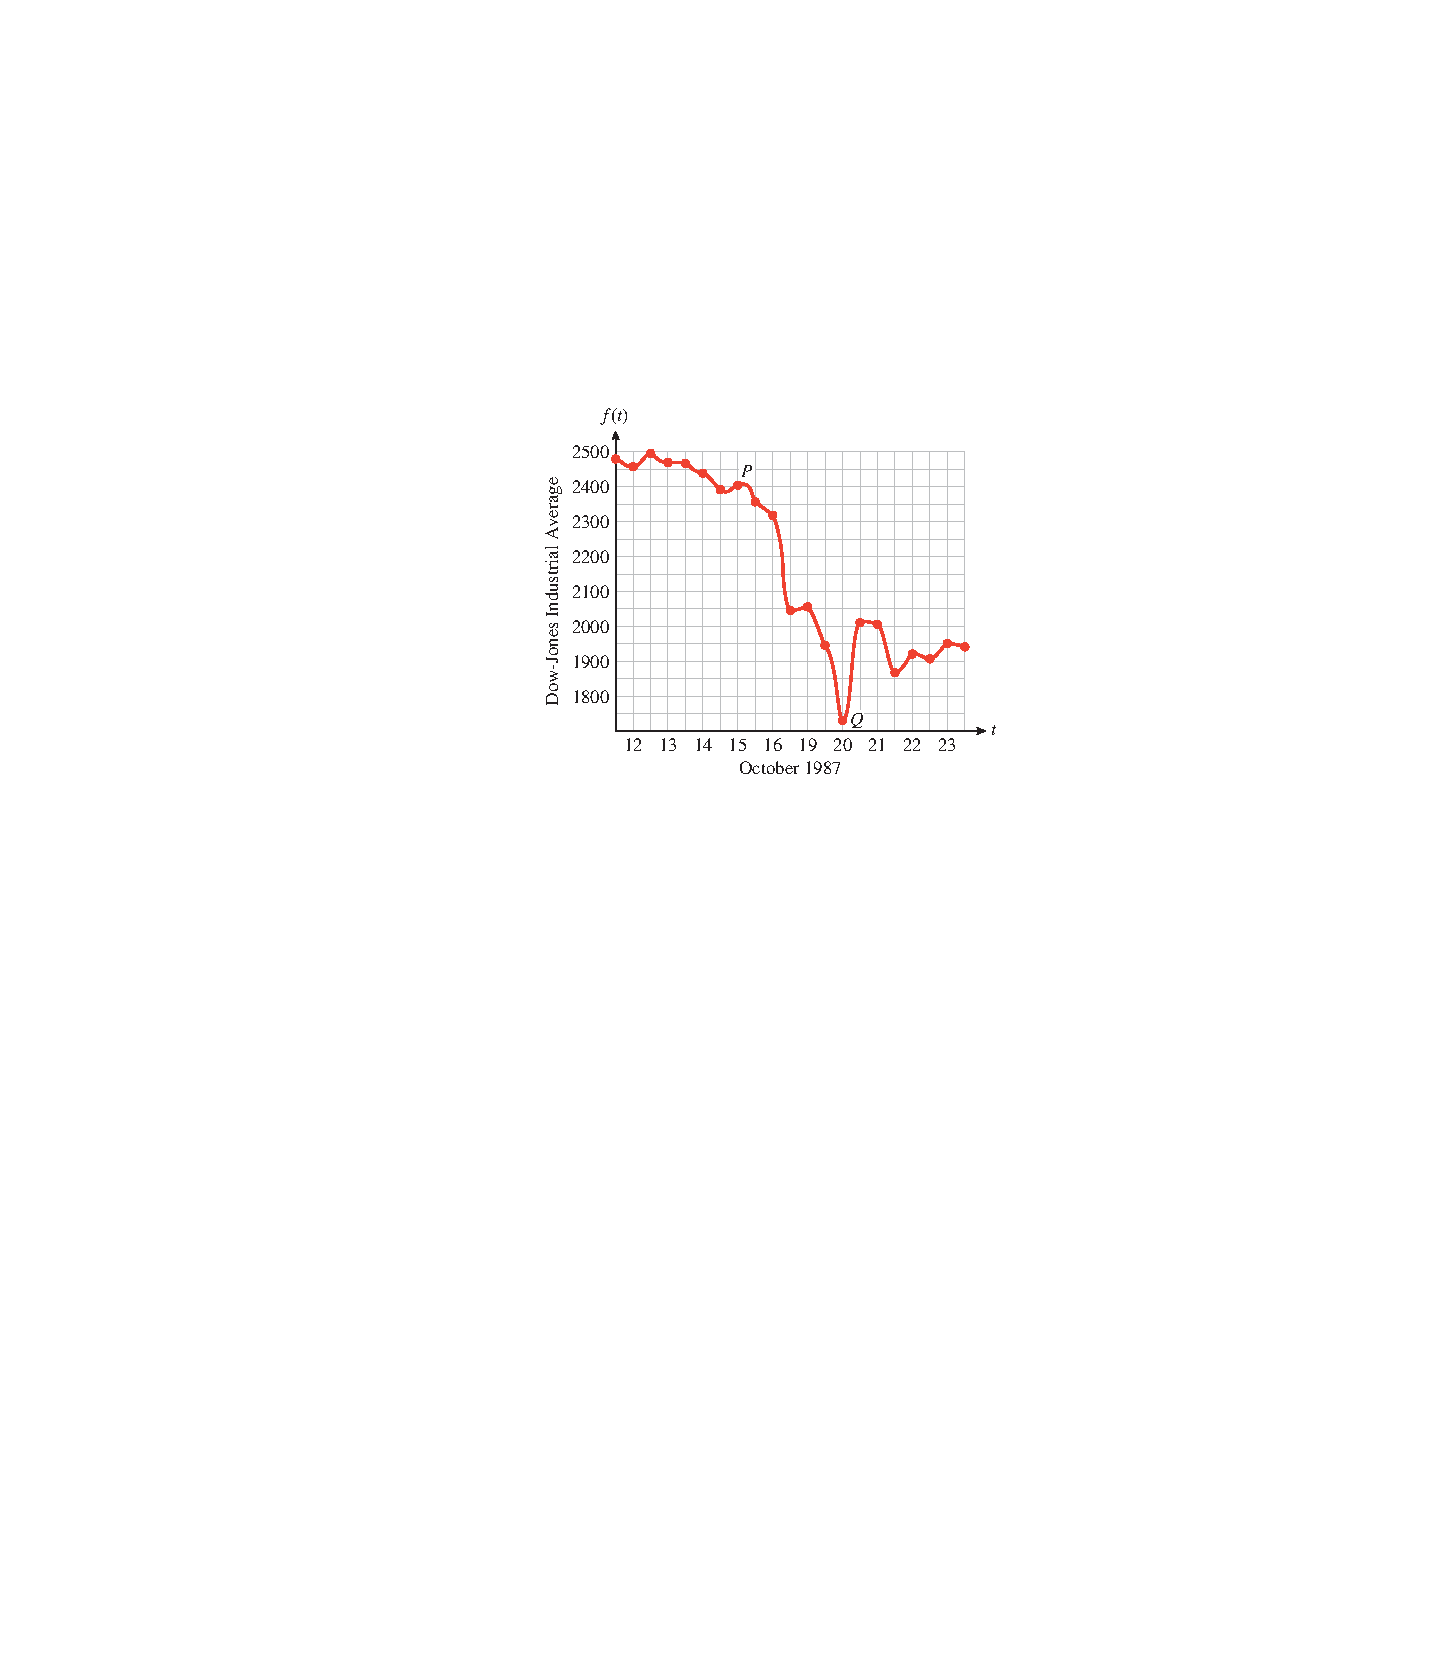
\includegraphics[width=0.80\textwidth,]{images/fig-DJIA.pdf}\caption{\label{fig-DJIA}}
\end{figure}
\par
The values of the input variable, time, are displayed on the horizontal axis, and the values of the output variable, DJIA, are displayed on the vertical axis. There is no formula that gives the DJIA for a particular day; but it is still a function, defined by its graph. The value of \(f(t)\) is specified by the vertical coordinate of the point with the given t-coordinate.
%
\begin{example}[]\label{example-DJIA}
\leavevmode%
\begin{enumerate}[label=*\alph**]
\item\hypertarget{li-1}{}The coordinates of point \(P\) in \hyperref[fig-DJIA]{Figure~\ref{fig-DJIA}} are \((15, 2412)\). What do the coordinates tell you about the function \(f\)?\item\hypertarget{li-2}{}If the DJIA was 1726 at noon on October 20, what can you say about the graph of \(f\)?\end{enumerate}
\par\medskip\noindent%
\textbf{Solution.}\quad \leavevmode%
\begin{enumerate}[label=*\alph**]
\item\hypertarget{li-3}{}The coordinates of point P tell us that \(f(15) = 2412\), so the DJIA was 2412 at noon on October 15.\item\hypertarget{li-4}{}We can say that \(f(20) = 1726\), so the point \((20, 1726)\) lies on the graph of \(f\). This point is labeled \(Q\) in \hyperref[fig-DJIA]{Figure~\ref{fig-DJIA}}.\end{enumerate}
\end{example}
\par
Thus, the coordinates of each point on the graph of the function represent a pair of corresponding
values of the two variables. In general, we can make the following statement.%
\typeout{************************************************}
\typeout{Paragraphs  Graph of a Function}
\typeout{************************************************}
\paragraph[Graph of a Function]{Graph of a Function}\label{paragraphs-1}
The point \((a, b)\) lies on the graph of the function \(f\) if and only if \(f(a)=b\).
%
\begin{example}[]\label{example-function-graph}
\hyperref[fig-function]{Figure~\ref{fig-function}} shows the graph of a function \(g\).
    \leavevmode%
\begin{enumerate}[label=*\alph**]
\item\hypertarget{li-5}{}Find \(g(−2)\) and \(g(5)\).\item\hypertarget{li-6}{}For what value(s) of \(t\) is \(g(t) = −2\)?\item\hypertarget{li-7}{}What is the largest, or maximum, value of \(g(t)\)? For what value of \(t\) does the function take on its maximum value?\item\hypertarget{li-8}{}On what intervals is \(g\) increasing?\end{enumerate}
%
\leavevmode%
\begin{figure}
\centering
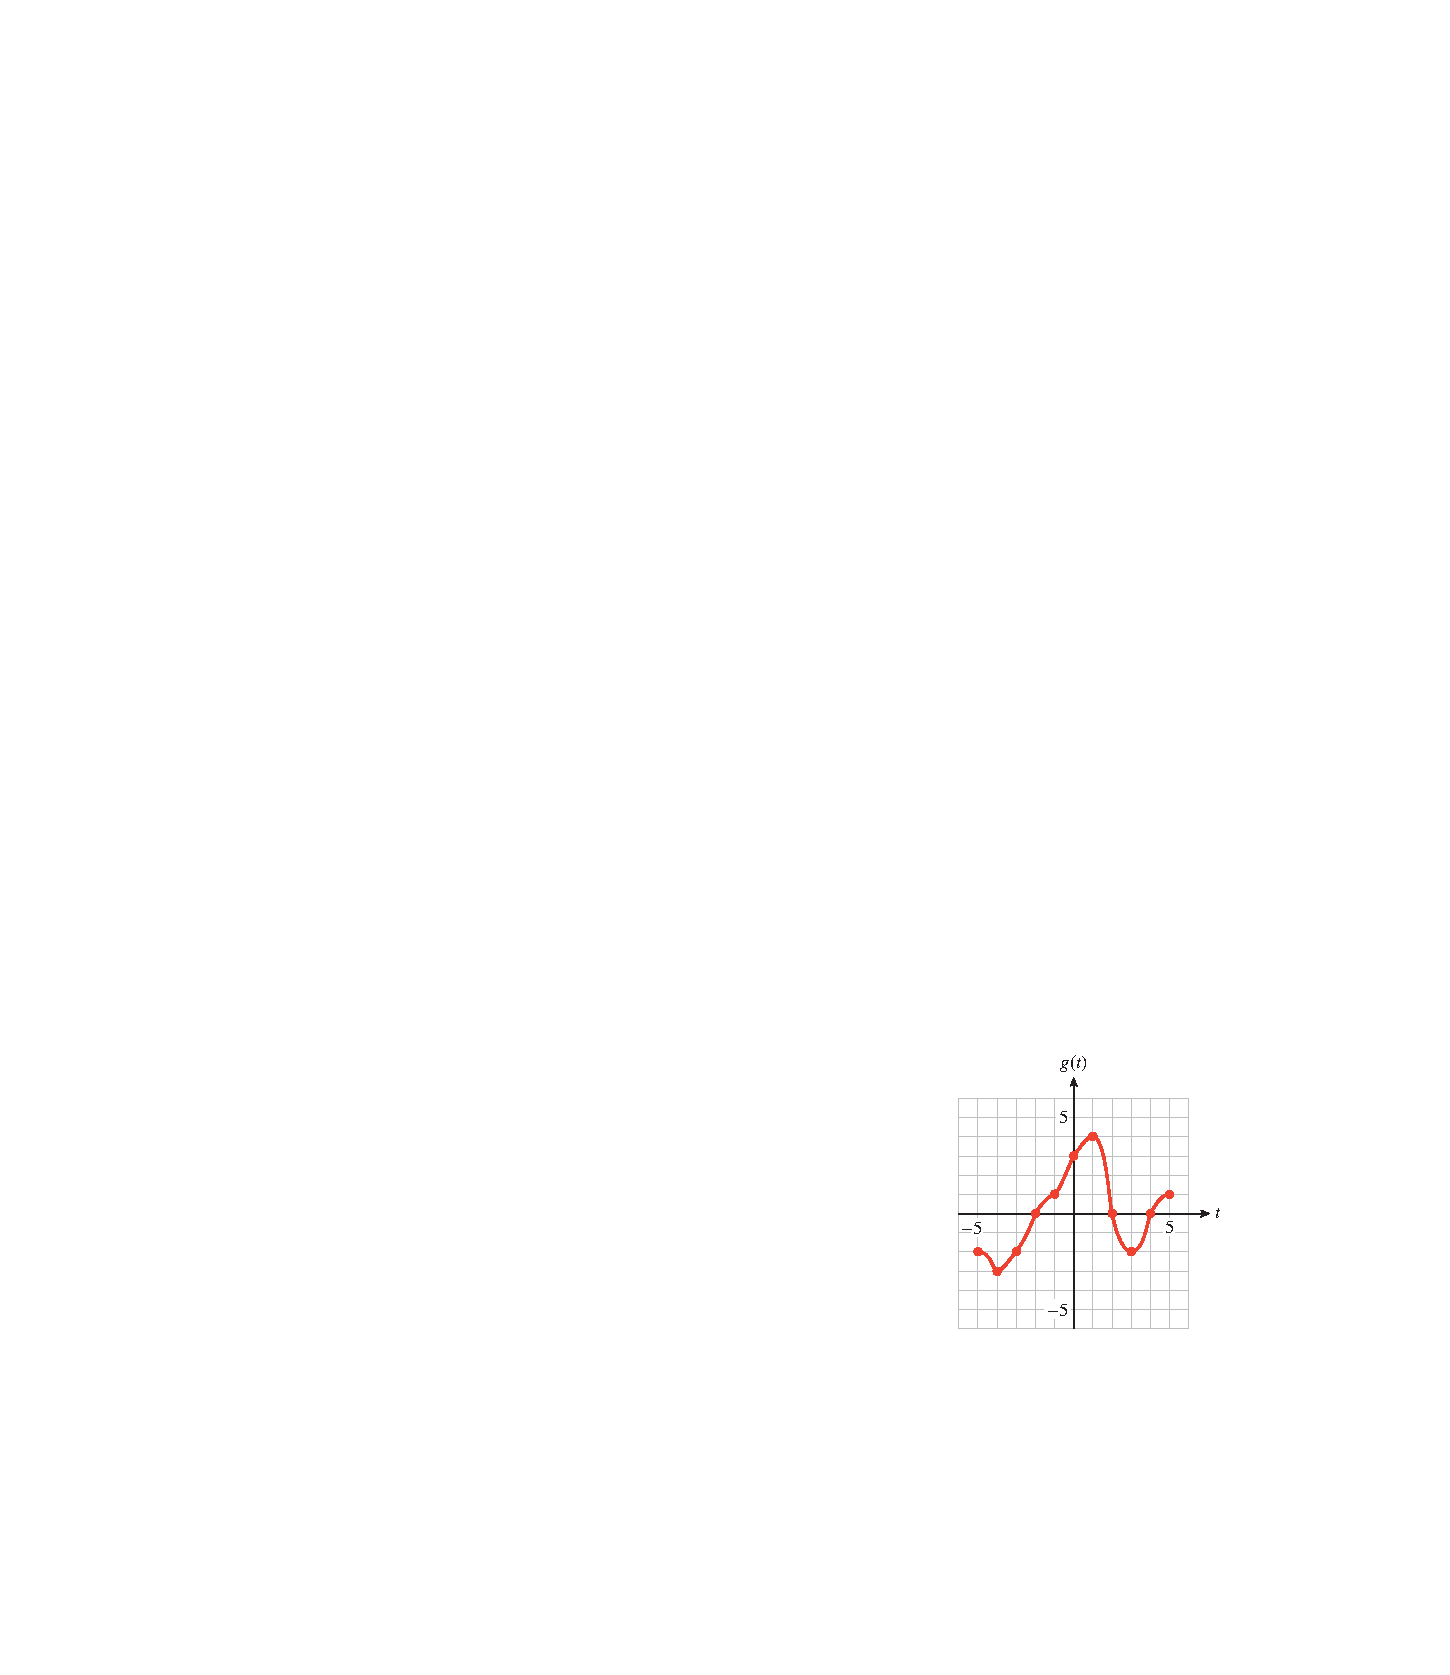
\includegraphics[width=0.60\textwidth,]{images/fig-function.pdf}\caption{\label{fig-function}}
\end{figure}
\par\medskip\noindent%
\textbf{Solution.}\quad \leavevmode%
\begin{enumerate}[label=*\alph**]
\item\hypertarget{li-9}{}To find \(g(−2)\), we look for the point with \(t\)-coordinate \(−2\). The point \((−2, 0)\) lies on the graph of \(g\), so \(g(−2) = 0\). Similarly, the point \((5, 1)\) lies on the graph, so \(g(5) = 1\).\item\hypertarget{li-10}{}We look for points on the graph with \(y\)-coordinate \(−2\). Because the points \((−5, −2)\), \((−3, −2)\), and \((3, −2)\) lie on the graph, we know that \(g(−5) = −2\), \(g(−3) = −2\), and \(g(3) = −2\). Thus, the \(t\)-values we want are \(−5\), \(−3\), and \(3\).\item\hypertarget{li-11}{}The highest point on the graph is \((1, 4)\), so the largest \(y\)-value is \(4\). Thus, the maximum value of \(g(t)\) is \(4\), and it occurs when \(t = 1\).\item\hypertarget{li-12}{}A graph is increasing if the \(y\)-values get larger as we read from left to right. The graph of \(g\) is increasing for \(t\)-values between \(−4\) and \(1\), and between \(3\) and \(5\). Thus, \(g\) is increasing on the intervals \((−4, 1)\) and \((3, 5)\).\end{enumerate}
\end{example}
\begin{exercise}\label{exercise-function-graph}

    Refer to the graph of the function \(g\) shown in \hyperref[fig-function]{Figure~\ref{fig-function}} in \hyperref[example-function-graph]{Example~\ref{example-function-graph}}.
    \leavevmode%
\begin{enumerate}[label=*\alph**]
\item\hypertarget{li-13}{}Find \(g(0)\).\item\hypertarget{li-14}{}For what value(s) of \(t\) is \(g(t) = 0\)?\item\hypertarget{li-15}{}What is the smallest, or minimum, value of \(g(t)\)? For what value of \(t\) does the function take on its minimum value?\item\hypertarget{li-16}{}On what intervals is \(g\) decreasing?\end{enumerate}
\end{exercise}
\begin{remark}[
\includegraphics[width=0.8\textwidth,]{images/icon-GC.pdf}Finding Coordinates with a Graphing Calculator]\label{remark-1}
We can use the 
\includegraphics[width=0.12\textwidth,]{images/icon-trace.pdf} feature of the calculator to find the coordinates of points on a graph. For example, graph the equation \(y = −2.6x − 5.4\) in the window%
\leavevmode%
\begin{table}
\centering
\begin{tabular}{lll}
Xmin\(=-5\)&&Xmax\(=4.4\)\tabularnewline[0pt]
Ymin\(=-20\)&&Ymax\(=15\)
\end{tabular}
\end{table}
\leavevmode%
\begin{figure}
\centering
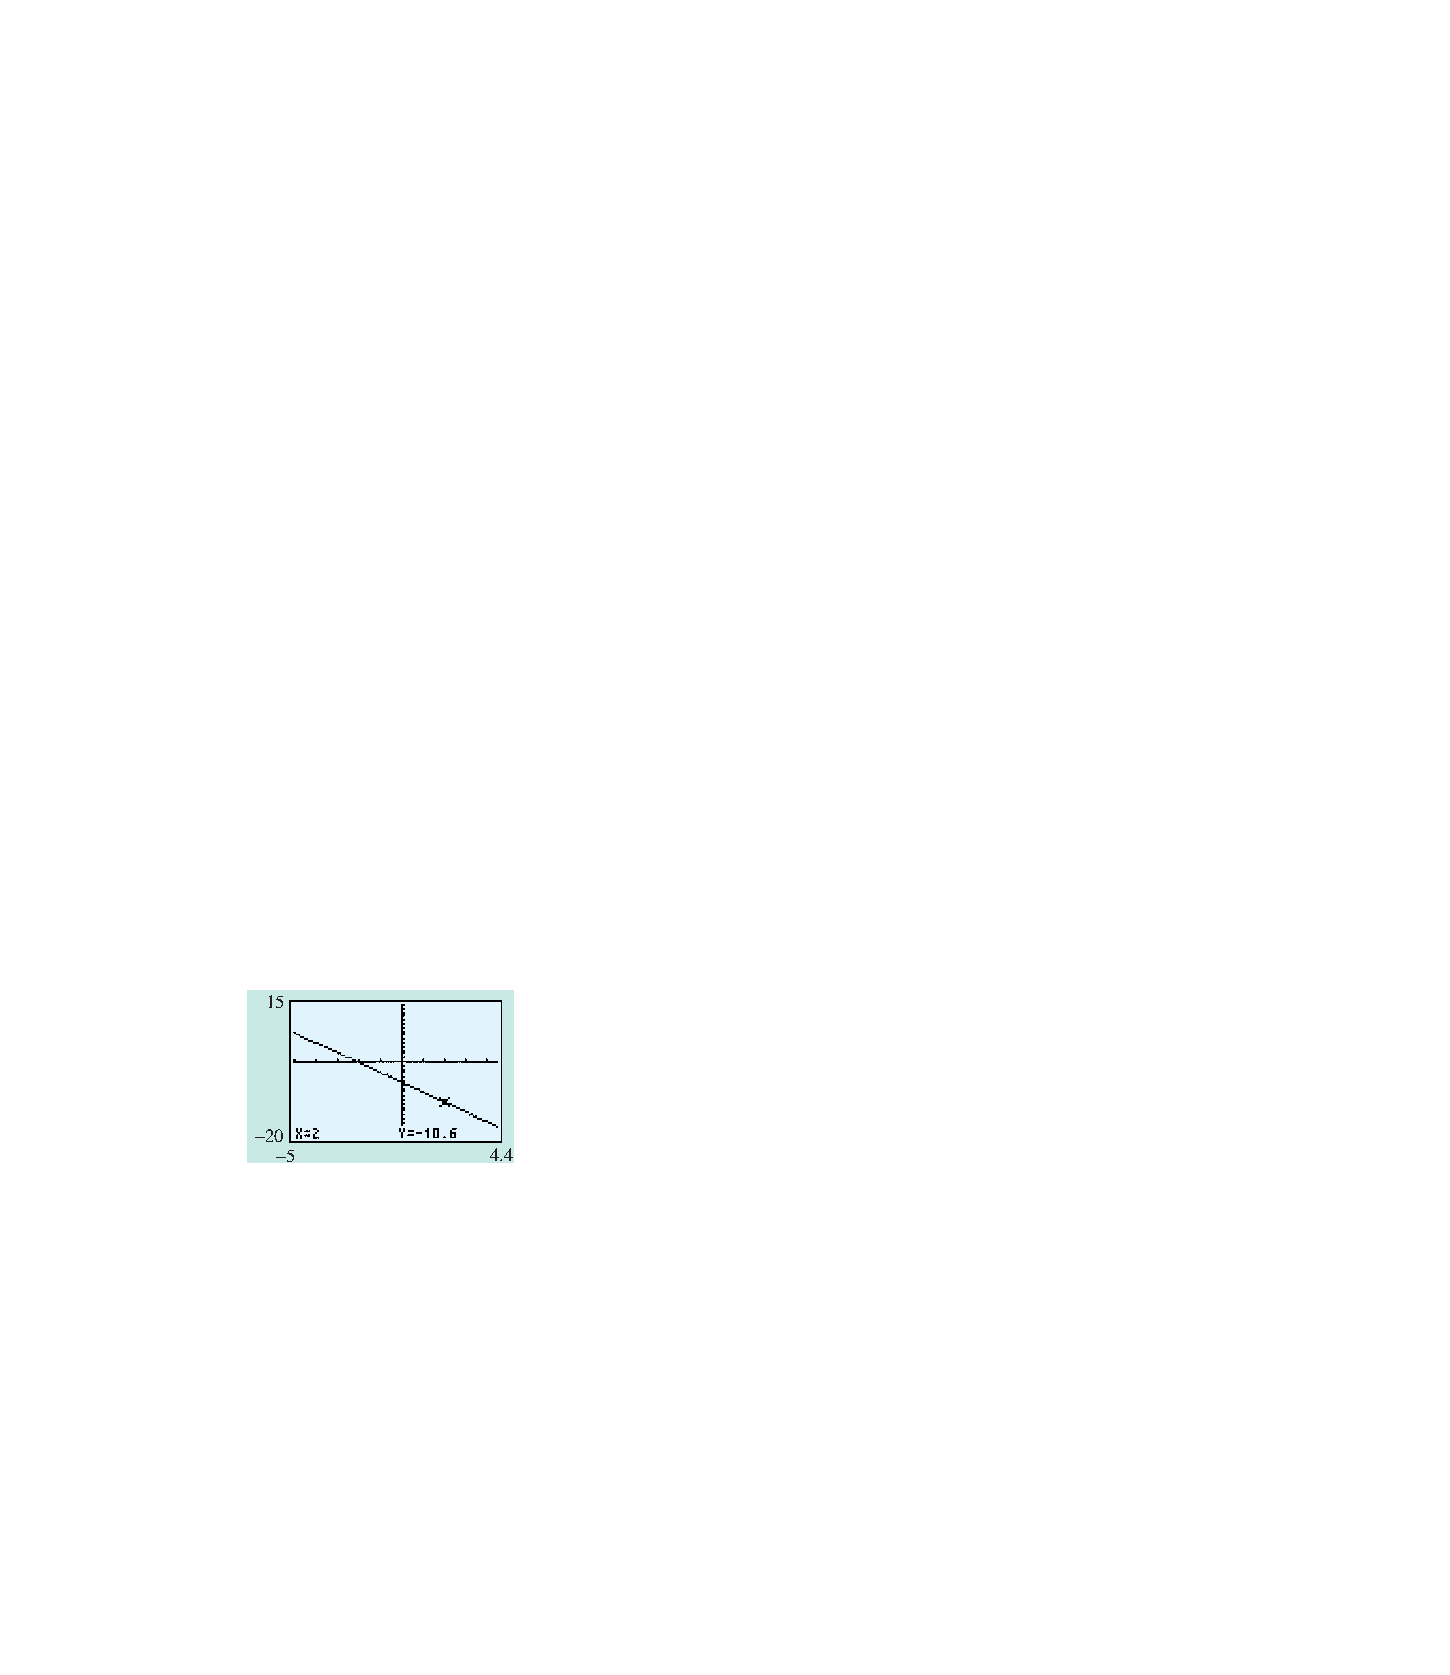
\includegraphics[width=0.60\textwidth,]{images/fig-GC-trace.pdf}\caption{\label{fig-GC-trace}}
\end{figure}
\par
Press 
\includegraphics[width=0.12\textwidth,]{images/icon-trace.pdf}, and a “bug” begins flashing on the display. The coordinates of the bug appear at the bottom of the display, as shown in \hyperref[fig-GC-trace]{Figure~\ref{fig-GC-trace}}. Use the left and right arrows to move the bug along the graph. You can check that the coordinates of the point \((2, −10.6)\) do satisfy the equation \(y = −2.6x − 5.4\).%
\par
The points identified by the Trace bug depend on the window settings and on the type of calculator. If we want to find the \(y\)-coordinate for a particular \(x\)-value, we enter the \(x\)-coordinate of the desired point and press 
\includegraphics[width=0.11\textwidth,]{images/icon-enter.pdf}.%
\end{remark}
\typeout{************************************************}
\typeout{Subsection 1.1.2 Constructing the Graph of a Function}
\typeout{************************************************}
\subsection[Constructing the Graph of a Function]{Constructing the Graph of a Function}\label{subsection-2}
Although some functions are defined by their graphs, we can also construct graphs for
functions described by tables or equations. We make these graphs the same way we graph
equations in two variables: by plotting points whose coordinates satisfy the equation.%
\begin{example}[]\label{example-graph-square-root}
Graph the function \(f(x) = \sqrt{x + 4}\).%
\par\medskip\noindent%
\textbf{Solution.}\quad Choose several convenient values for \(x\) and evaluate the function to find the corresponding \(f(x)\)-values. For this function we cannot choose \(x\)-values less than \(−4\), because the square root of a negative number is not a real number. 
    \begin{equation*}f(\alert{−4}) =\sqrt{\alert{−4} + 4}=\sqrt{0}= 0\end{equation*}
    \begin{equation*}f(\alert{−3}) =\sqrt{\alert{−3} + 4}=\sqrt{1}= 1\end{equation*}
    \begin{equation*}f(\alert{0}) =\sqrt{\alert{0} + 4}=\sqrt{4}=2\end{equation*}
    \begin{equation*}f(\alert{2}) =\sqrt{\alert{2} + 4}=\sqrt{6}\approx 2.45\end{equation*}
    \begin{equation*}f(\alert{5}) =\sqrt{\alert{5} + 4}=\sqrt{9}=3\end{equation*}
    The results are shown in the table.%
\leavevmode%
\begin{figure}
\centering
\pushValignCaptionBottom[b]{minipage}{.50\textwidth}{%
\centering% horizontal alignment 
\begin{tabular}{AcAcA}\hrulethick
\(x\)%
&\(f(x)\)%
\tabularnewline\hrulethin
\(-4\)&\(0\)\tabularnewline\hrulethin
\(-3\)&\(1\)\tabularnewline\hrulethin
\(0\)&\(2\)\tabularnewline\hrulethin
\(2\)&\(\sqrt{6}\)\tabularnewline\hrulethin
\(5\)&\(3\)\tabularnewline\hrulethin
\end{tabular}
}% end body 
{}% caption 
\pushValignCaptionBottom[b]{minipage}{.50\textwidth}{%
\centering% horizontal alignment 
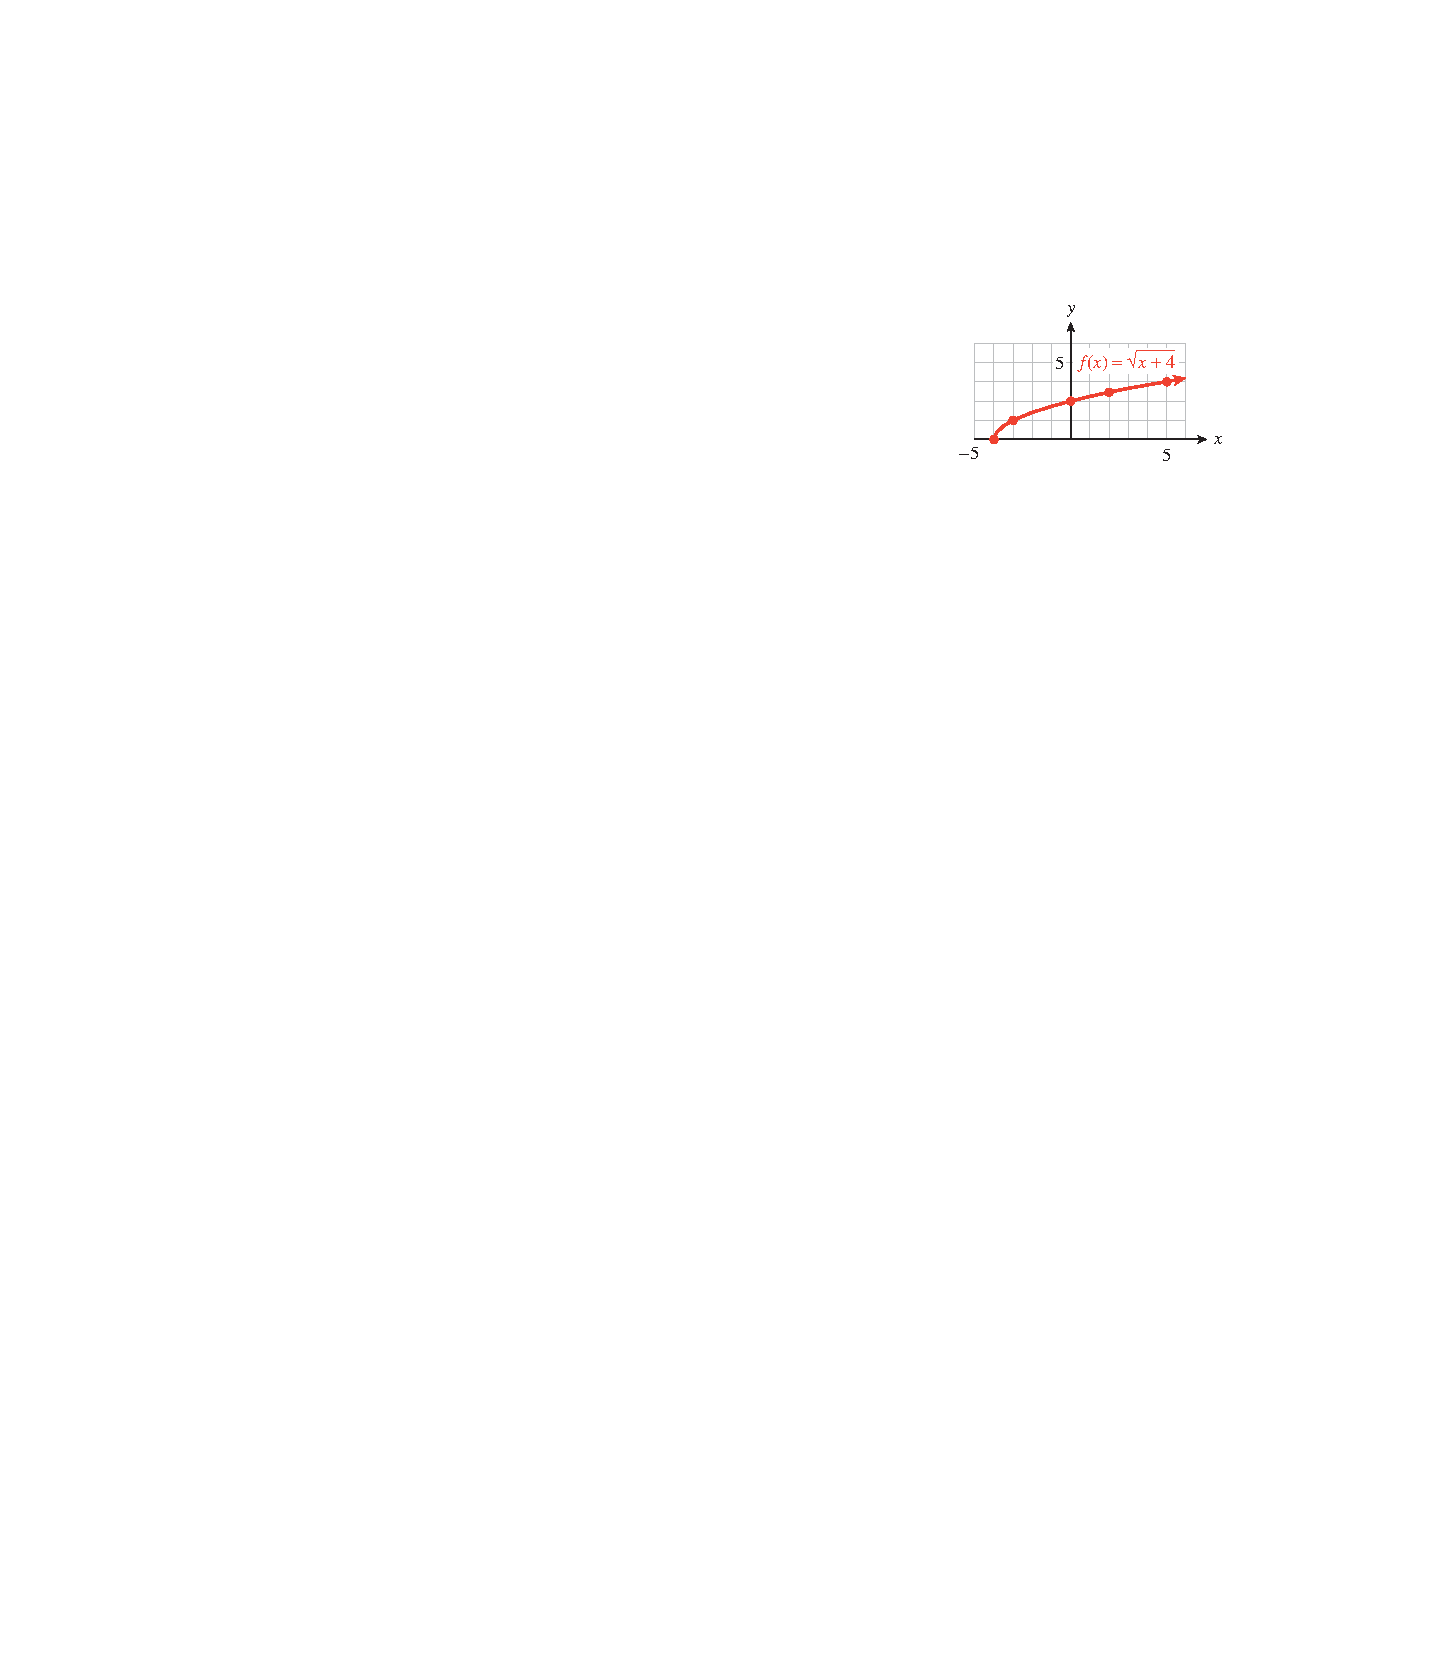
\includegraphics[width=\textwidth,]{images/fig-sq-root.pdf}}% end body 
{\captionof{figure}{\label{fig-sq-root}}
}% caption 
\popValignCaptionBottom
\end{figure}
\end{example}
\begin{remark}[
\includegraphics[width=0.8\textwidth,]{images/icon-GC.pdf}Using a Calculator to Graph a Function]\label{remark-2}
We can also use a graphing calculator to obtain a table and graph for the function in \hyperref[example-graph-square-root]{Example~\ref{example-graph-square-root}}. We graph a function just as we graphed an equation. For this function, we enter \begin{equation*}Y_1 = \sqrt{~^~}(X+4)\end{equation*}
    and press 
\includegraphics[width=0.12\textwidth,]{images/icon-zoom.pdf}\(6\) for the standard window. (See {$\langle\langle$appendix-b$\rangle\rangle$}  for details.) The calculator’s graph is shown in \hyperref[fig-GC-sq-root]{Figure~\ref{fig-GC-sq-root}}.%
\leavevmode%
\begin{figure}
\centering
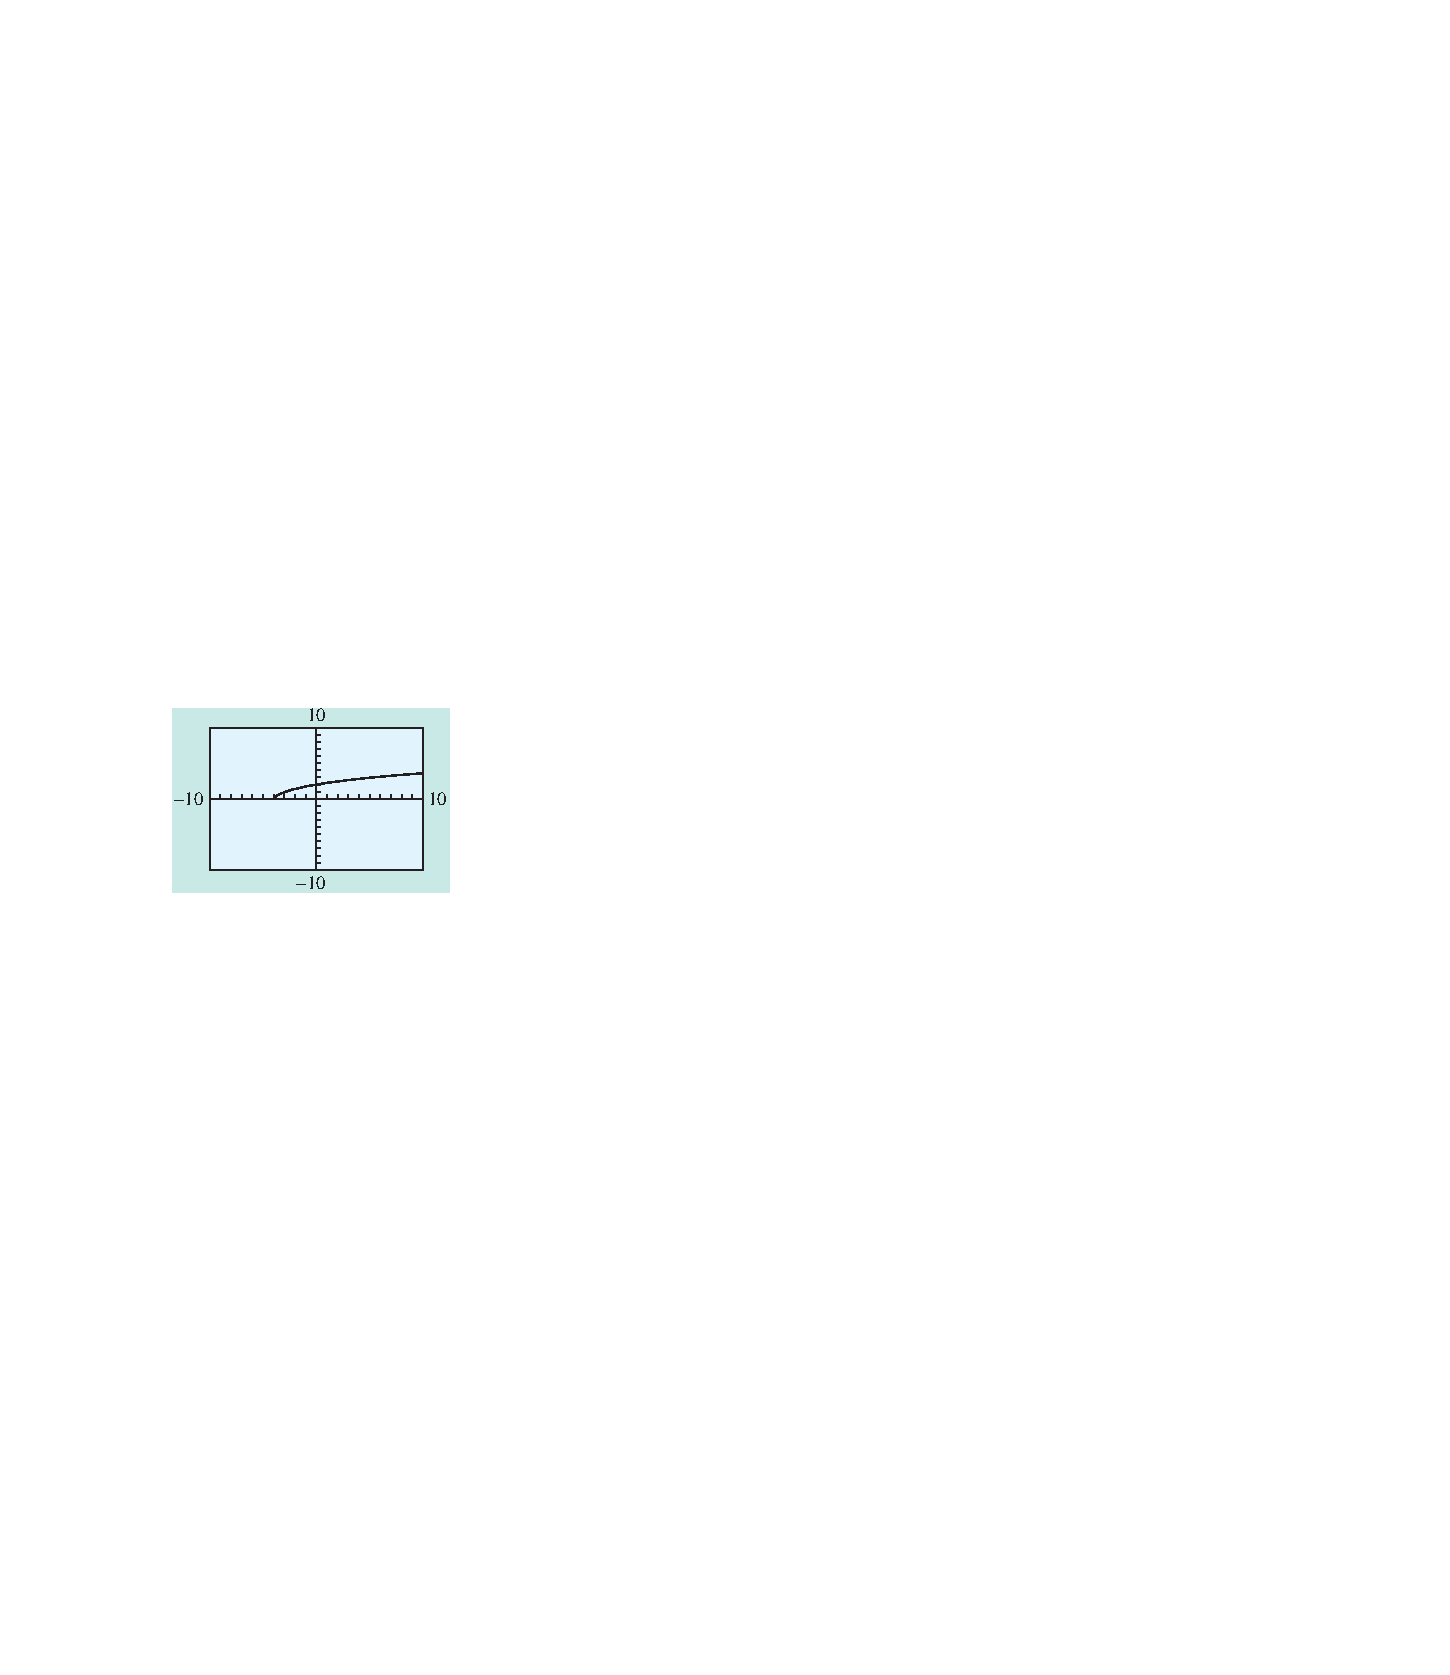
\includegraphics[width=0.50\textwidth,]{images/fig-GC-sq-root.pdf}\caption{\label{fig-GC-sq-root}}
\end{figure}
\end{remark}
\begin{exercise}\label{exercise-cubic-graph}
\begin{equation*}f(x) = x^3 − 2\end{equation*}\leavevmode%
\begin{enumerate}[label=*\alph**]
\item\hypertarget{li-17}{}Complete the table of values and sketch a graph of the function.
    \leavevmode%
\begin{table}
\centering
\begin{tabular}{AcAcAcAcAcAcAcAcA}\hrulethick
\(x\)&\(-2\)&\(-1\)&\(-\frac{1}{2}\)&\(0\)&\(\frac{1}{2}\)&\(1\)&\(2\)\tabularnewline\hrulethin
\(f(x)\)&%
&%
&%
&%
&%
&%
&%
\tabularnewline\hrulethin
\end{tabular}
\end{table}
\item\hypertarget{li-18}{}Use your calculator to make a table of values and graph the function.\end{enumerate}
\end{exercise}
\typeout{************************************************}
\typeout{Subsection 1.1.3 The Vertical Line Test}
\typeout{************************************************}
\subsection[The Vertical Line Test]{The Vertical Line Test}\label{subsection-3}
In a function, two different outputs cannot be related to the same input. This restriction means that two different ordered pairs cannot have the same first coordinate. What does it mean for the graph of the function?%
\par
Consider the graph shown in \hyperref[fig-vertical-line-test]{Figure~\ref{fig-vertical-line-test}}a. Every vertical line intersects the graph in at most one point, so there is only one point on the graph for each \(x\)-value. This graph represents a function. In \hyperref[fig-vertical-line-test]{Figure~\ref{fig-vertical-line-test}}b, however, the line \(x = 2\) intersects the graph at two points, \((2, 1)\) and \((2, 4)\). Two different \(y\)-values, \(1\) and \(4\), are related to the same \(x\)-value, \(2\). This graph cannot be the graph of a function.%
\leavevmode%
\begin{figure}
\centering
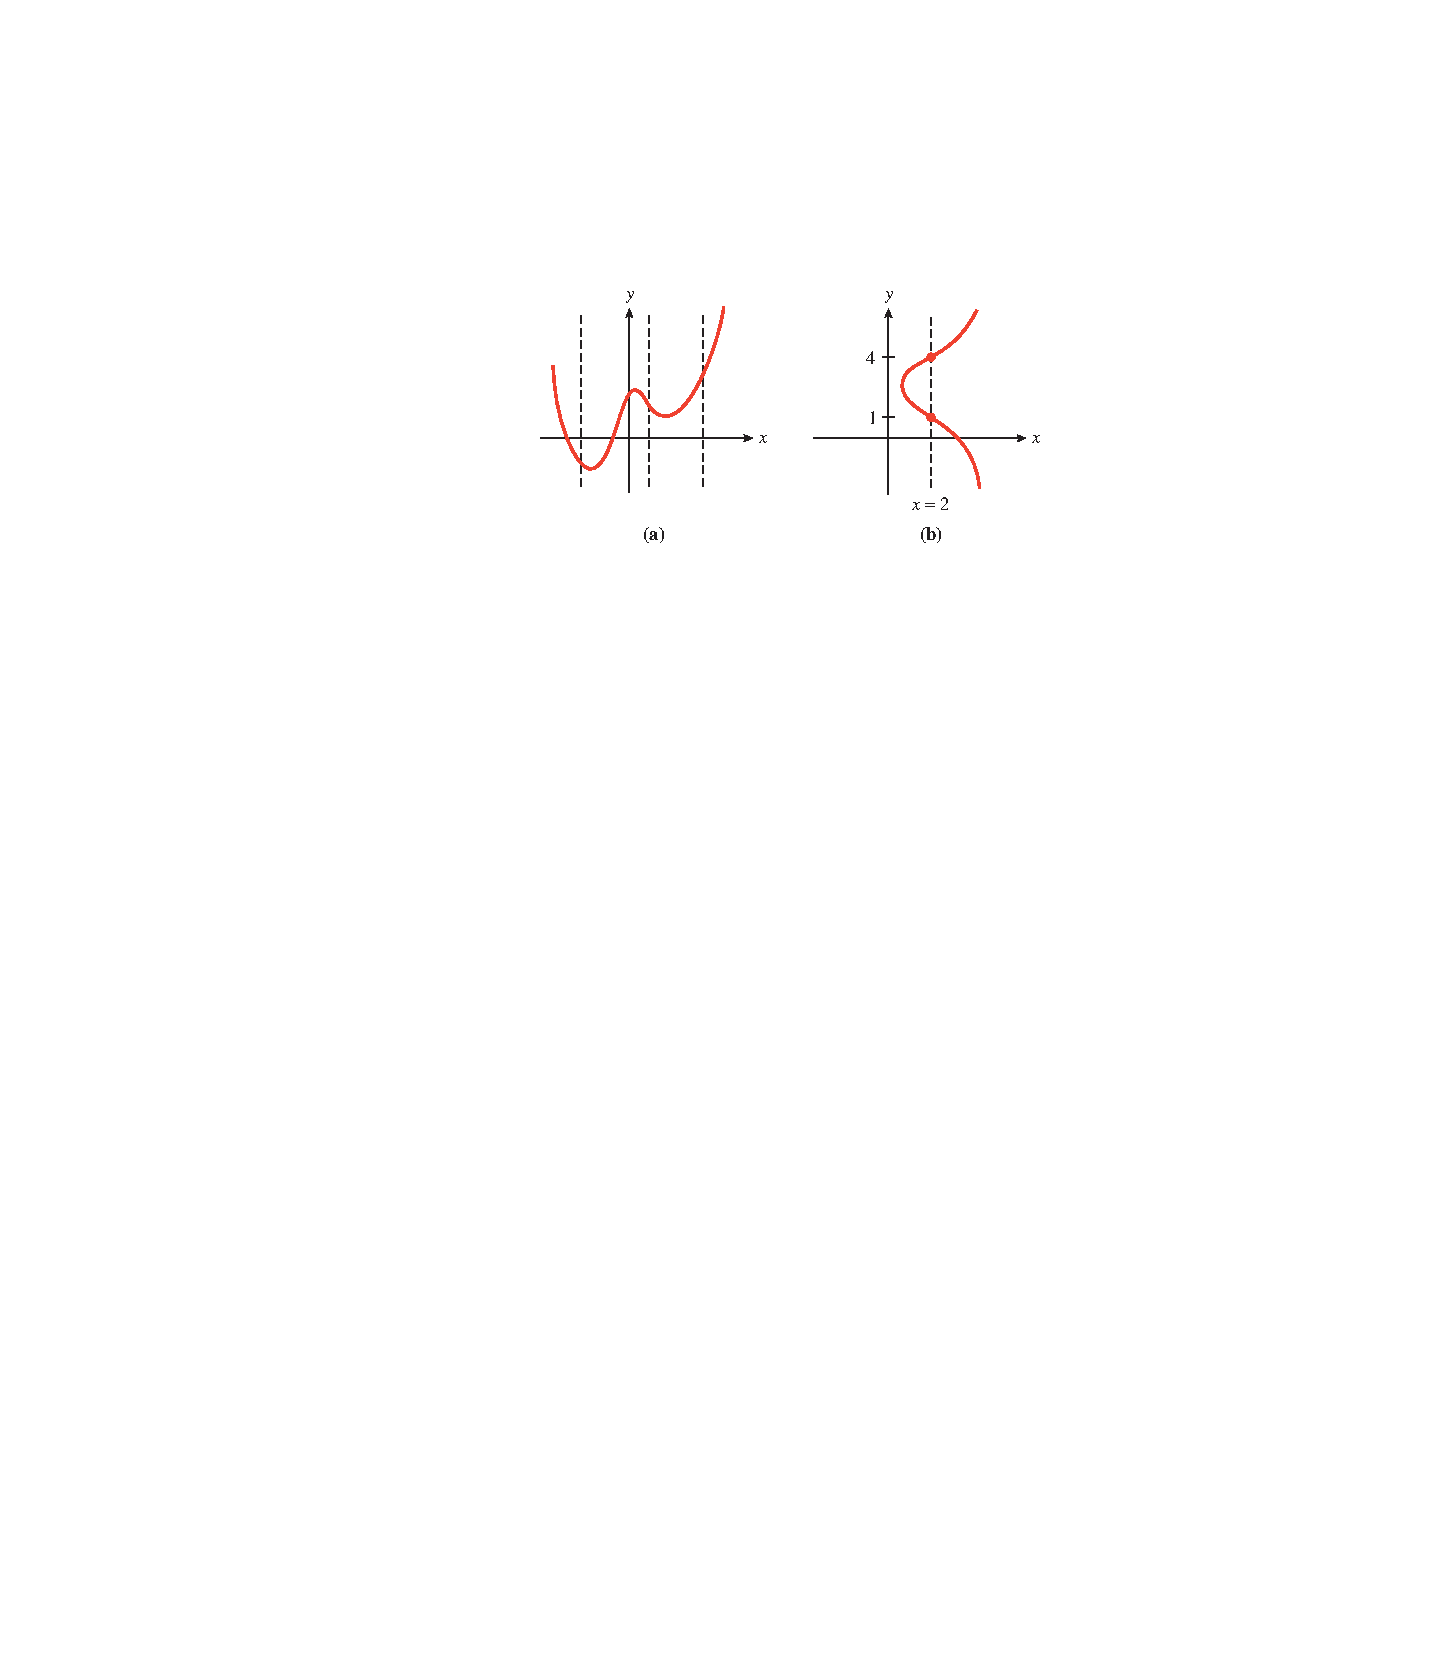
\includegraphics[width=0.90\textwidth,]{images/fig-vertical-line-test.pdf}\caption{\label{fig-vertical-line-test}}
\end{figure}
\par
We summarize these observations as follows.%
\typeout{************************************************}
\typeout{Paragraphs  The Vertical Line Test}
\typeout{************************************************}
\paragraph[The Vertical Line Test]{The Vertical Line Test}\label{paragraphs-2}
A graph represents a function if and only if every vertical line intersects the graph in
at most one point.%
\begin{example}[]\label{example-vertical-line-test}
Use the vertical line test to decide which of the graphs in \hyperref[fig-vertical-line-test2]{Figure~\ref{fig-vertical-line-test2}}  represent functions.%
\leavevmode%
\begin{figure}
\centering
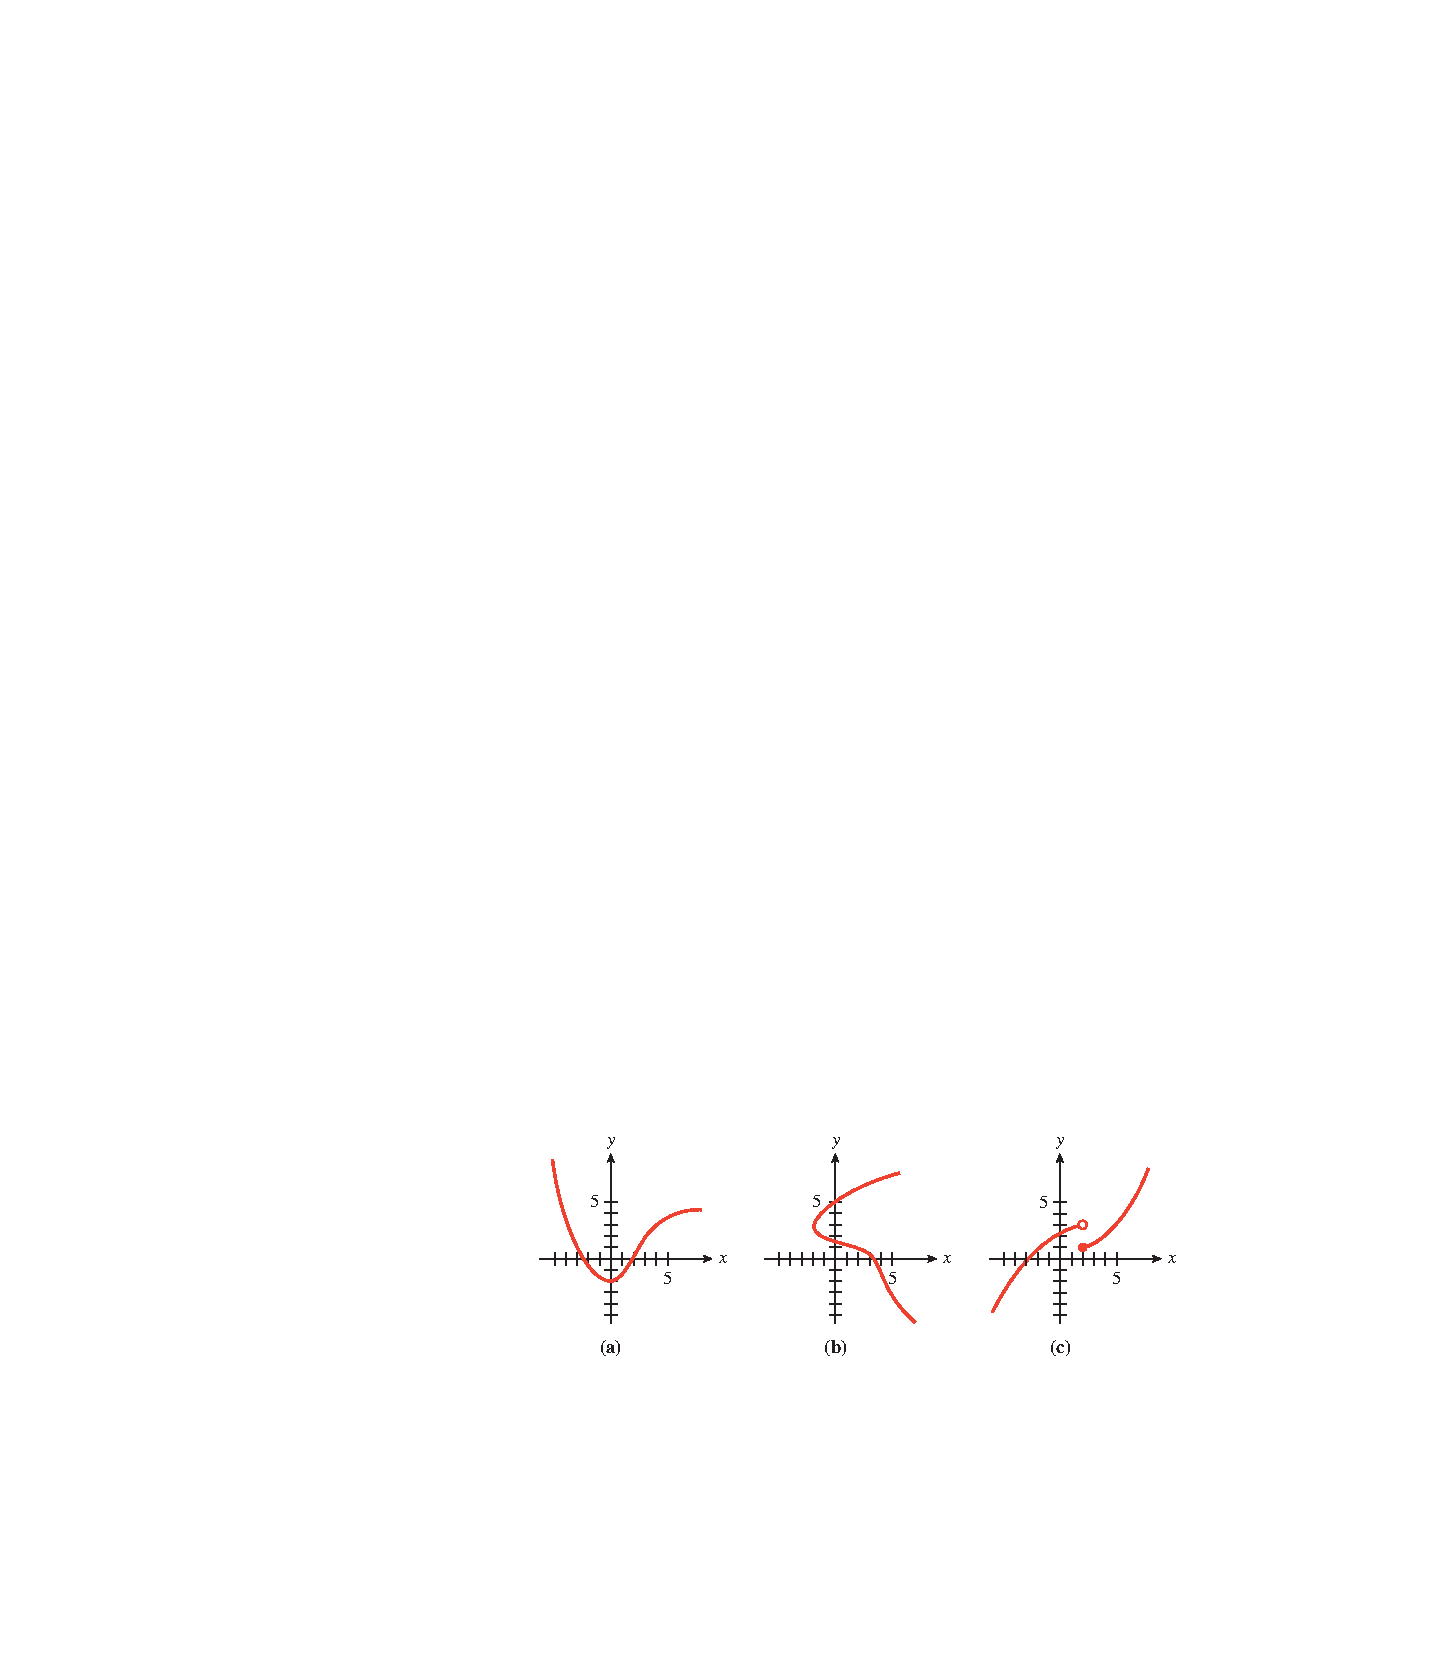
\includegraphics[width=0.90\textwidth,]{images/fig-vertical-line-test2.pdf}\caption{\label{fig-vertical-line-test2}}
\end{figure}
\par\medskip\noindent%
\textbf{Solution.}\quad 
    Graph (a) represents a function, because it passes the vertical line test. Graph (b) is not the graph of a function, because the vertical line at (for example) \(x = 1\) intersects the graph at two points. For graph (c), notice the break in the curve at \(x = 2\): The solid dot at \((2, 1)\) is the only point on the graph with \(x = 2\); the open circle at \((2, 3)\) indicates that \((2, 3)\) is not a point on the graph. Thus, graph (c) is a function, with \(f(2) = 1\).
\end{example}
\begin{exercise}\label{example-vertical-line-test3}
Use the vertical line test to determine which of the graphs in \hyperref[fig-vertical-line-test3]{Figure~\ref{fig-vertical-line-test3}} represent functions.
    \leavevmode%
\begin{figure}
\centering
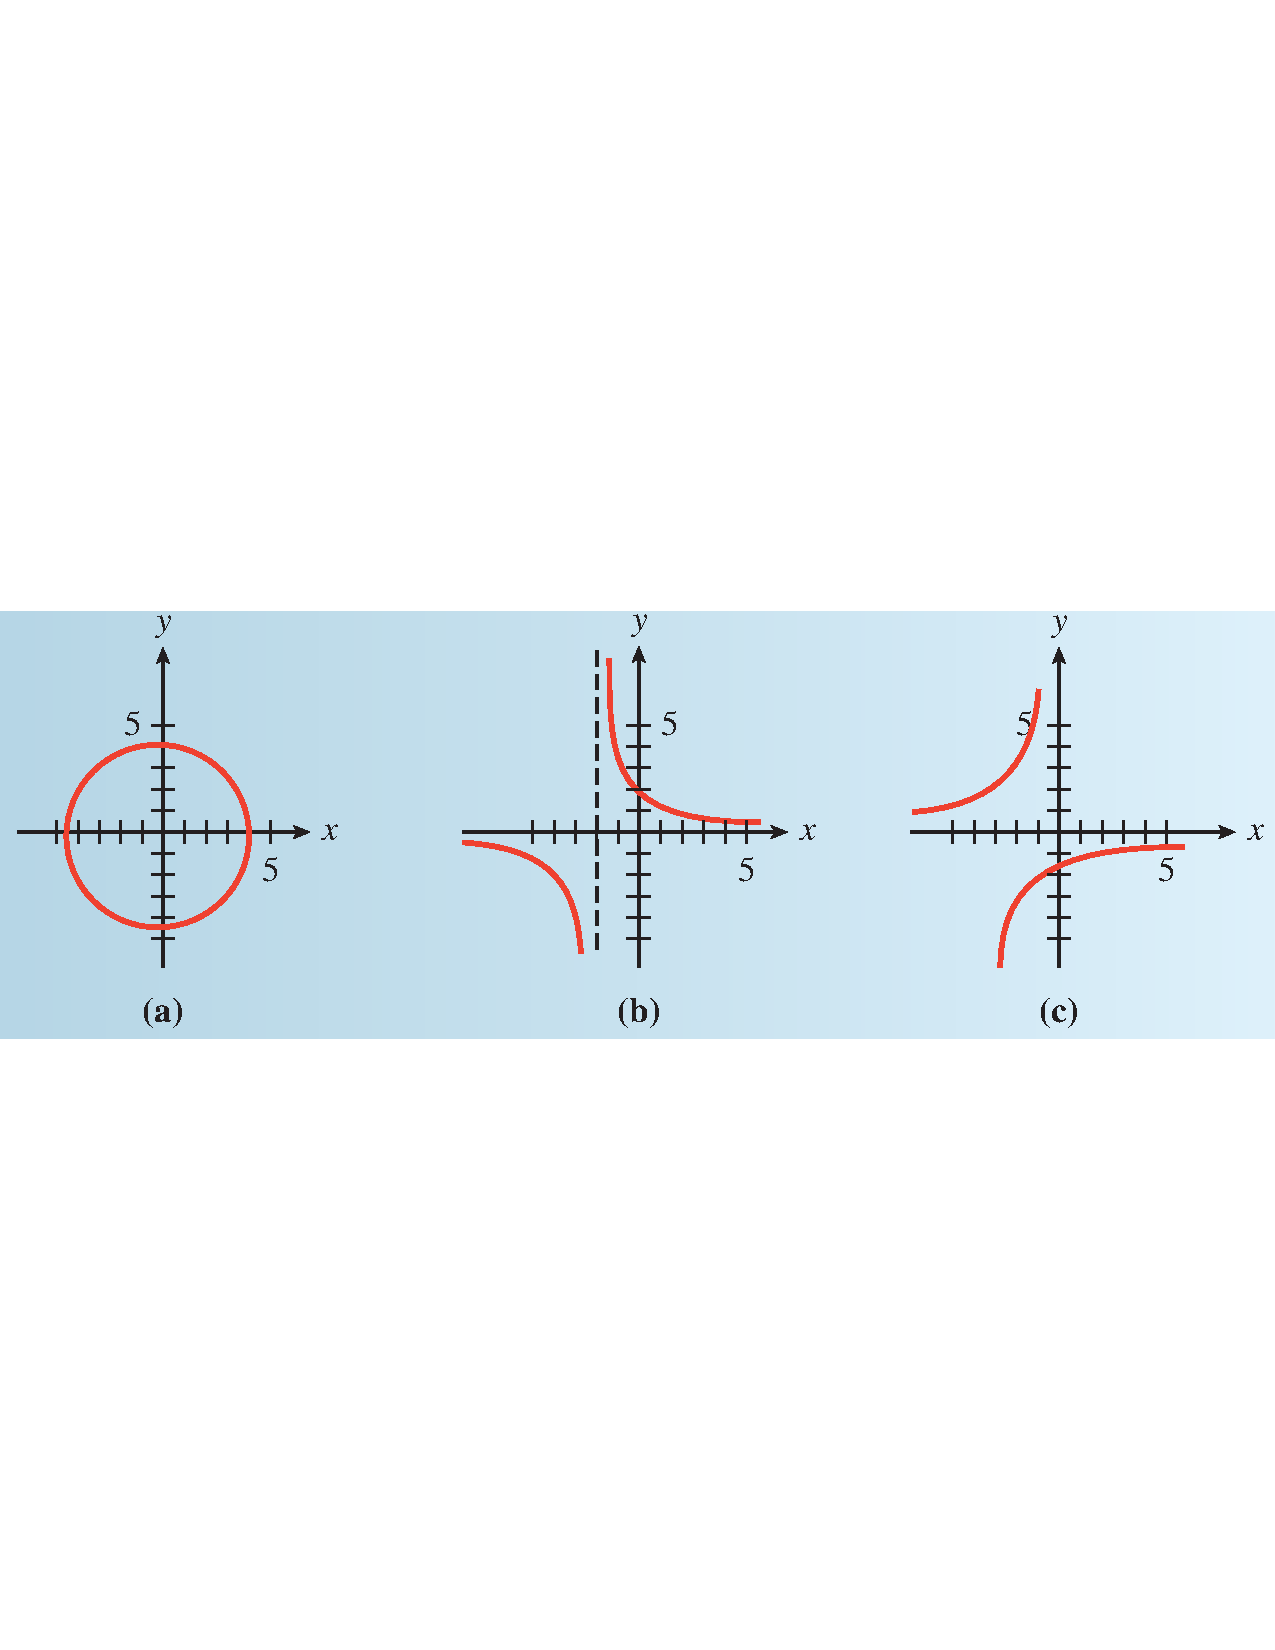
\includegraphics[width=0.100\textwidth,]{images/fig-vertical-line-test3.pdf}\caption{\label{fig-vertical-line-test3}}
\end{figure}
\end{exercise}
\typeout{************************************************}
\typeout{Subsection 1.1.4 Graphical Solution of Equations and Inequalities}
\typeout{************************************************}
\subsection[Graphical Solution of Equations and Inequalities]{Graphical Solution of Equations and Inequalities}\label{subsection-4}
The graph of an equation in two variables is just a picture of its solutions. When we read the coordinates of a point on the graph, we are reading a pair of \(x\)- and \(y\)-values that make the equation true. %
\leavevmode%
\begin{figure}
\centering
\pushValignCaptionBottom[b]{minipage}{.50\textwidth}{%
\parbox{\textwidth}{%
% horizontal alignment 
For example, the point \((2, 7)\) lies on the graph of \(y = 2x + 3\) shown in \hyperref[fig-function-graph]{Figure~\ref{fig-function-graph}} , so we know that the ordered pair \((2, 7)\) is a solution of the equation \(y = 2x + 3\). You can verify algebraically that \(x = \alert{2}\) and \(y = \alert{7}\) satisfy the equation: 
    \begin{equation*}\text{Does }~\alert{7} = 2 (\alert{2}) + 3\text{? Yes}\end{equation*}
    We can also say that \(x = 2\) is a solution of the one-variable equation \(2x + 3 = 7\). In fact, we can use the graph of \(y = 2x + 3\) to solve the equation \(2x + 3 = k\) for any value of \(k\). Thus, we can use graphs to find solutions to equations in one variable.}%
}% end body 
{}% caption 
\pushValignCaptionBottom[b]{minipage}{.50\textwidth}{%
\centering% horizontal alignment 
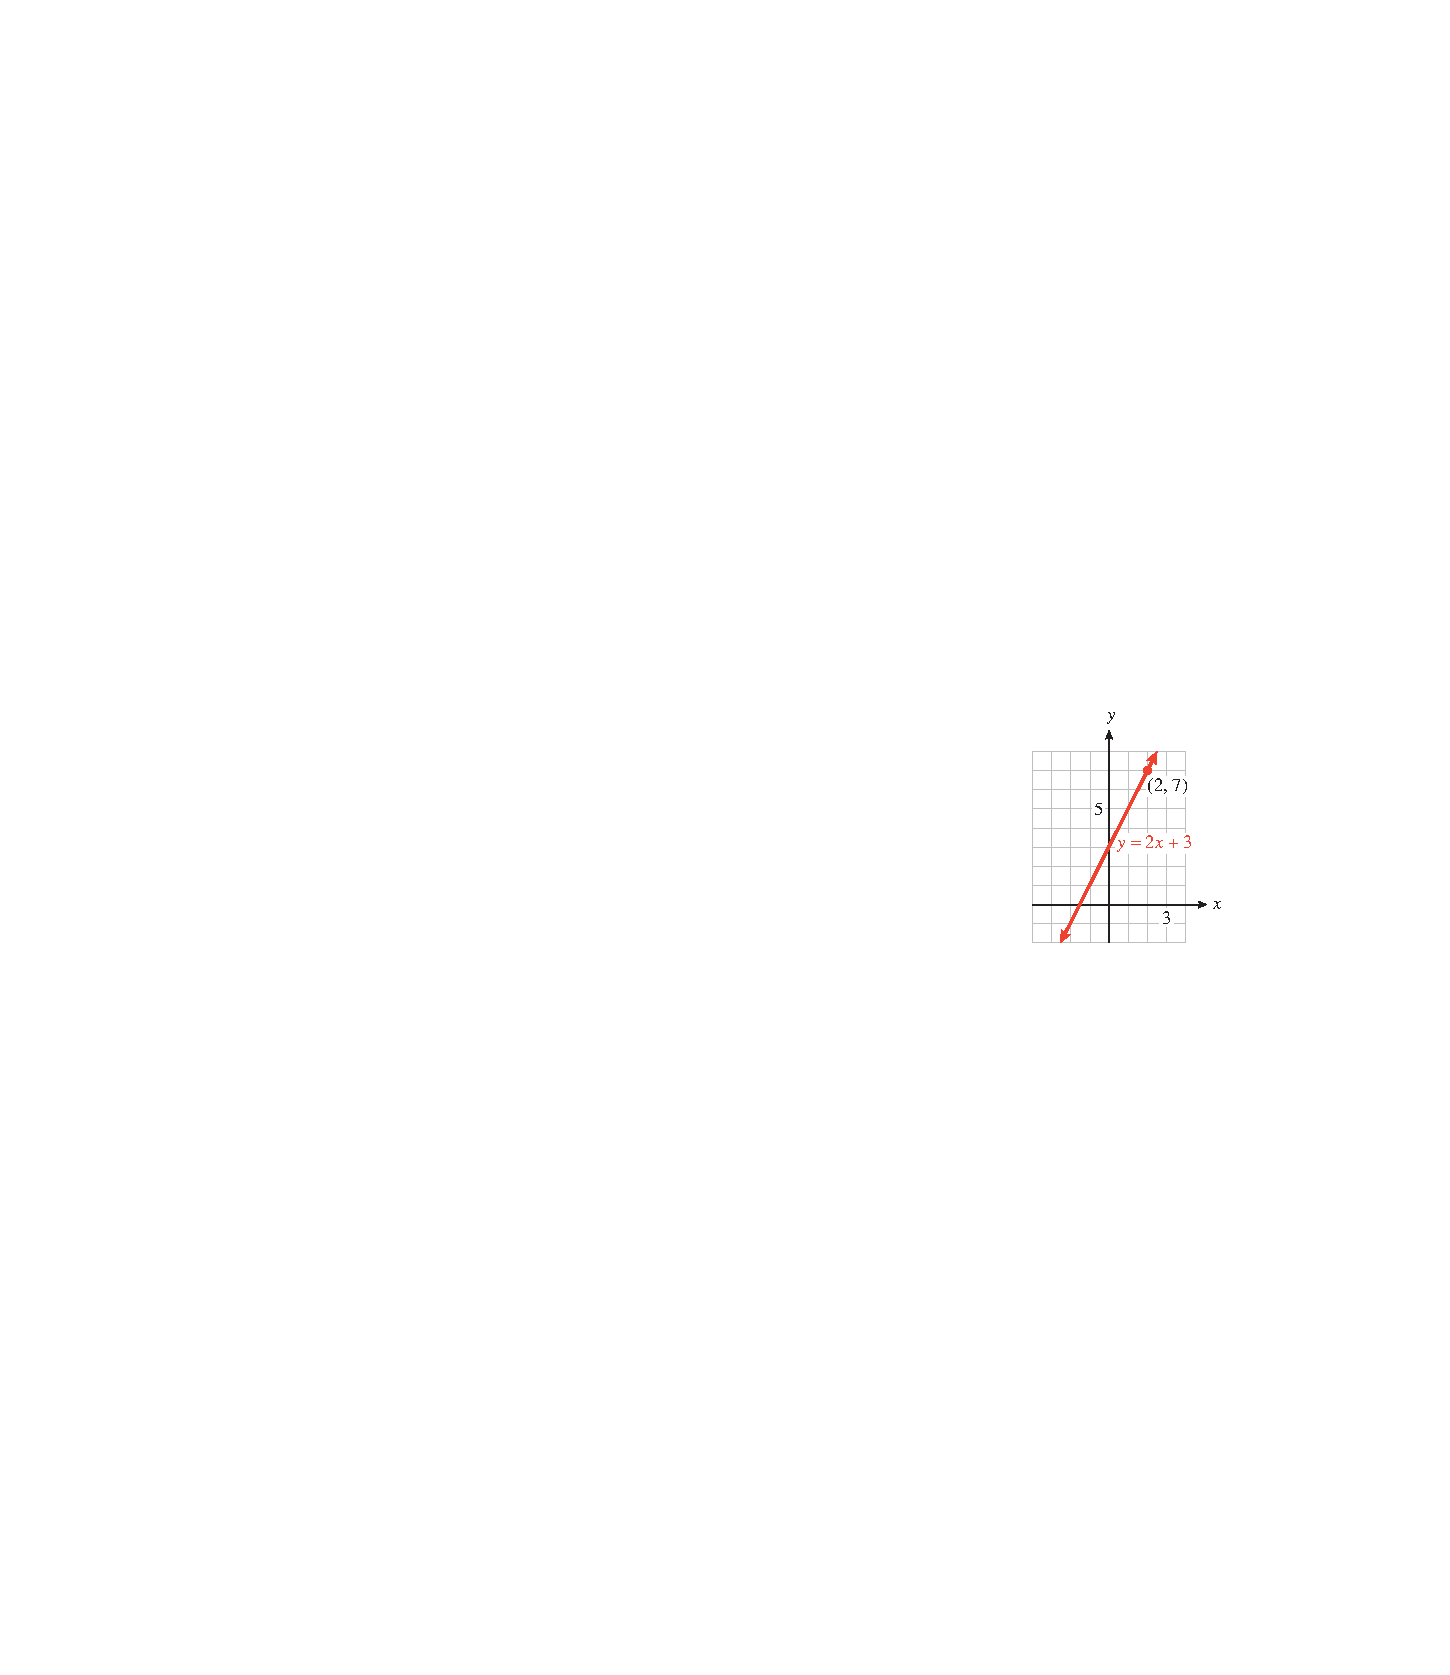
\includegraphics[width=\textwidth,]{images/fig-function-graph.pdf}}% end body 
{\captionof{figure}{\label{fig-function-graph}}
}% caption 
\popValignCaptionBottom
\end{figure}
\begin{example}[]\label{example-graph-to-solve}
Use the graph of \(y = 285 − 15x\) to solve the equation \(150 = 285 − 15x\).%
\par\medskip\noindent%
\textbf{Solution.}\quad \leavevmode%
\begin{figure}
\centering
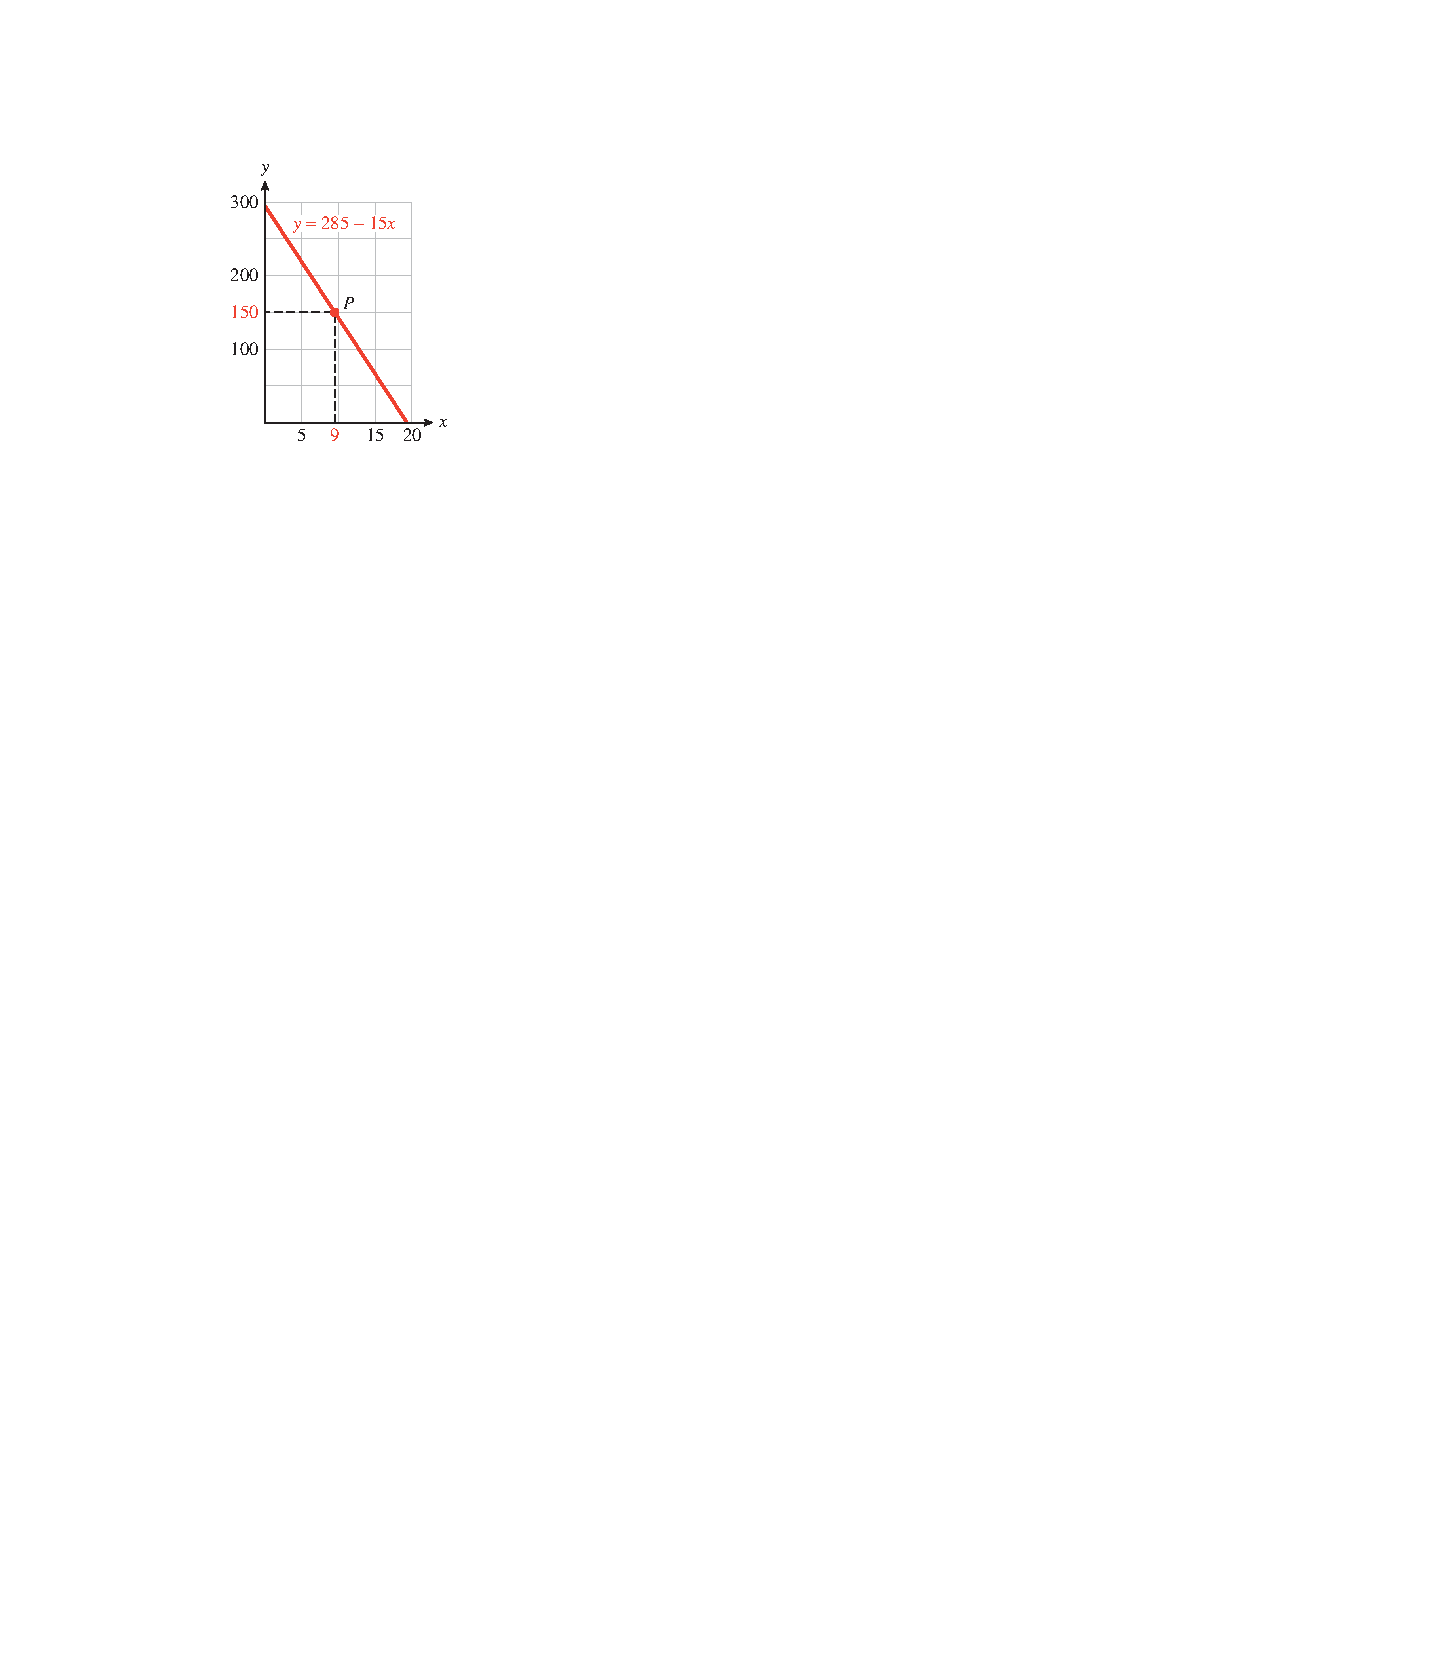
\includegraphics[width=0.50\textwidth,]{images/fig-graph-to-solve.pdf}\caption{\label{fig-graph-to-solve}}
\end{figure}
Begin by locating the point \(P\) on the graph for which \(y = 150\), as shown in \hyperref[fig-graph-to-solve]{Figure~\ref{fig-graph-to-solve}}. Now find the \(x\)-coordinate of point \(P\) by drawing an imaginary line from \(P\) straight down to the \(x\)-axis. The \(x\)-coordinate of \(P\) is \(x = 9\). Thus, \(P\) is the point \((9,150)\), and \(x = 9\) when \(y = 150\). The solution of the equation \(150 = 285 − 15x\) is \(x = 9\). You can verify the solution algebraically by substituting \(x = \alert{9}\) into the equation:%
\par
Does \(150 = 285 − 15(\alert{9})\)? %
\begin{equation*}285 − 15(\alert{9}) = 285 − 135 = 150. ~~\alert{Yes}\end{equation*}\end{example}
\par
The relationship between an equation and its graph is an important one. For the
previous example, make sure you understand that the following three statements are
equivalent:
%
\leavevmode%
\begin{enumerate}
\item\hypertarget{li-19}{}The point \((9, 150)\) lies on the graph of \(y = 285 − 15x\).\item\hypertarget{li-20}{}The ordered pair \((9, 150)\) is a solution of the equation \(y = 285 − 15x\).\item\hypertarget{li-21}{}\(x = 9\) is a solution of the equation \(150 = 285 − 15x\).\end{enumerate}
\begin{exercise}\label{exercise-graph-to-solve}
\leavevmode%
\begin{enumerate}[label=*\alph**]
\item\hypertarget{li-22}{}Use the graph of \(y = 30 − 8x\) shown in \hyperref[fig-graph-to-solve2]{Figure~\ref{fig-graph-to-solve2}} to solve the equation \begin{equation*}30 − 8x = 50\end{equation*}\item\hypertarget{li-23}{}Verify your solution algebraically.\end{enumerate}
\leavevmode%
\begin{figure}
\centering
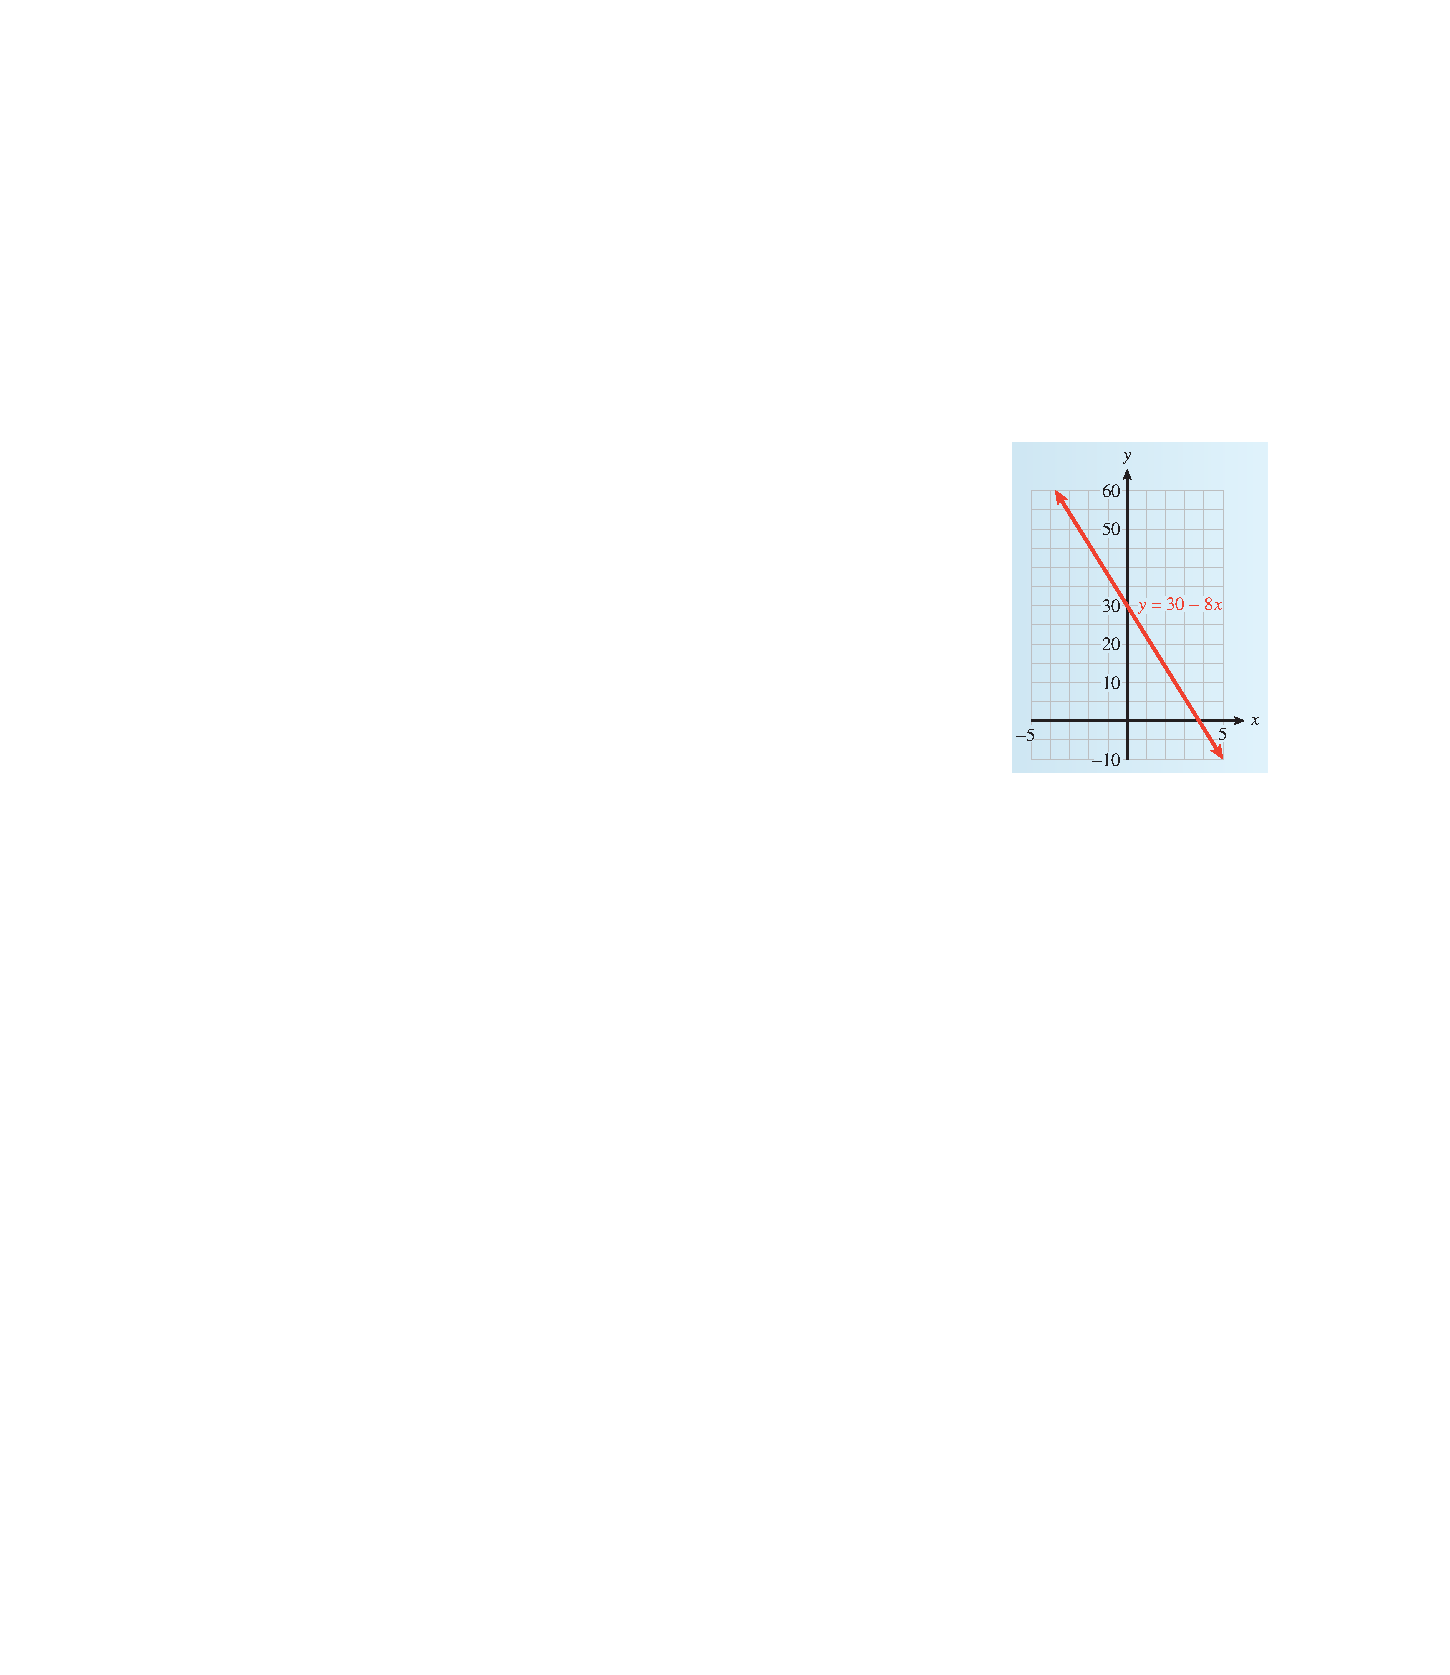
\includegraphics[width=0.50\textwidth,]{images/fig-graph-to-solve2.pdf}\caption{\label{fig-graph-to-solve2}}
\end{figure}
\end{exercise}
\leavevmode%
\begin{figure}
\centering
\pushValignCaptionBottom[b]{minipage}{.50\textwidth}{%
\parbox{\textwidth}{%
% horizontal alignment 
In a similar fashion, we can solve inequalities with a graph. Consider again the graph of \(y = 2x + 3\), shown in \hyperref[fig-graph-to-solve3]{Figure~\ref{fig-graph-to-solve3}}. We saw that \(x = 2\) is the solution of the equation \(2x + 3 = 7\). When we use \(x = 2\) as the input for the function \(f(x) = 2x + 3\), the output is \(y = 7\). Which input values for \(x\) produce output values greater than \(7\)? You can see in \hyperref[fig-graph-to-solve3]{Figure~\ref{fig-graph-to-solve3}} that \(x\)-values greater than \(2\) produce \(y\)-values greater than \(7\), because points on the graph with \(x\)-values greater than \(2\) have \(y\)-values greater than \(7\). Thus, the solutions of the inequality \(2x + 3 \gt 7\) are \(x\gt 2\). You can verify this result by solving the inequality algebraically.}%
}% end body 
{}% caption 
\pushValignCaptionBottom[b]{minipage}{.50\textwidth}{%
\centering% horizontal alignment 
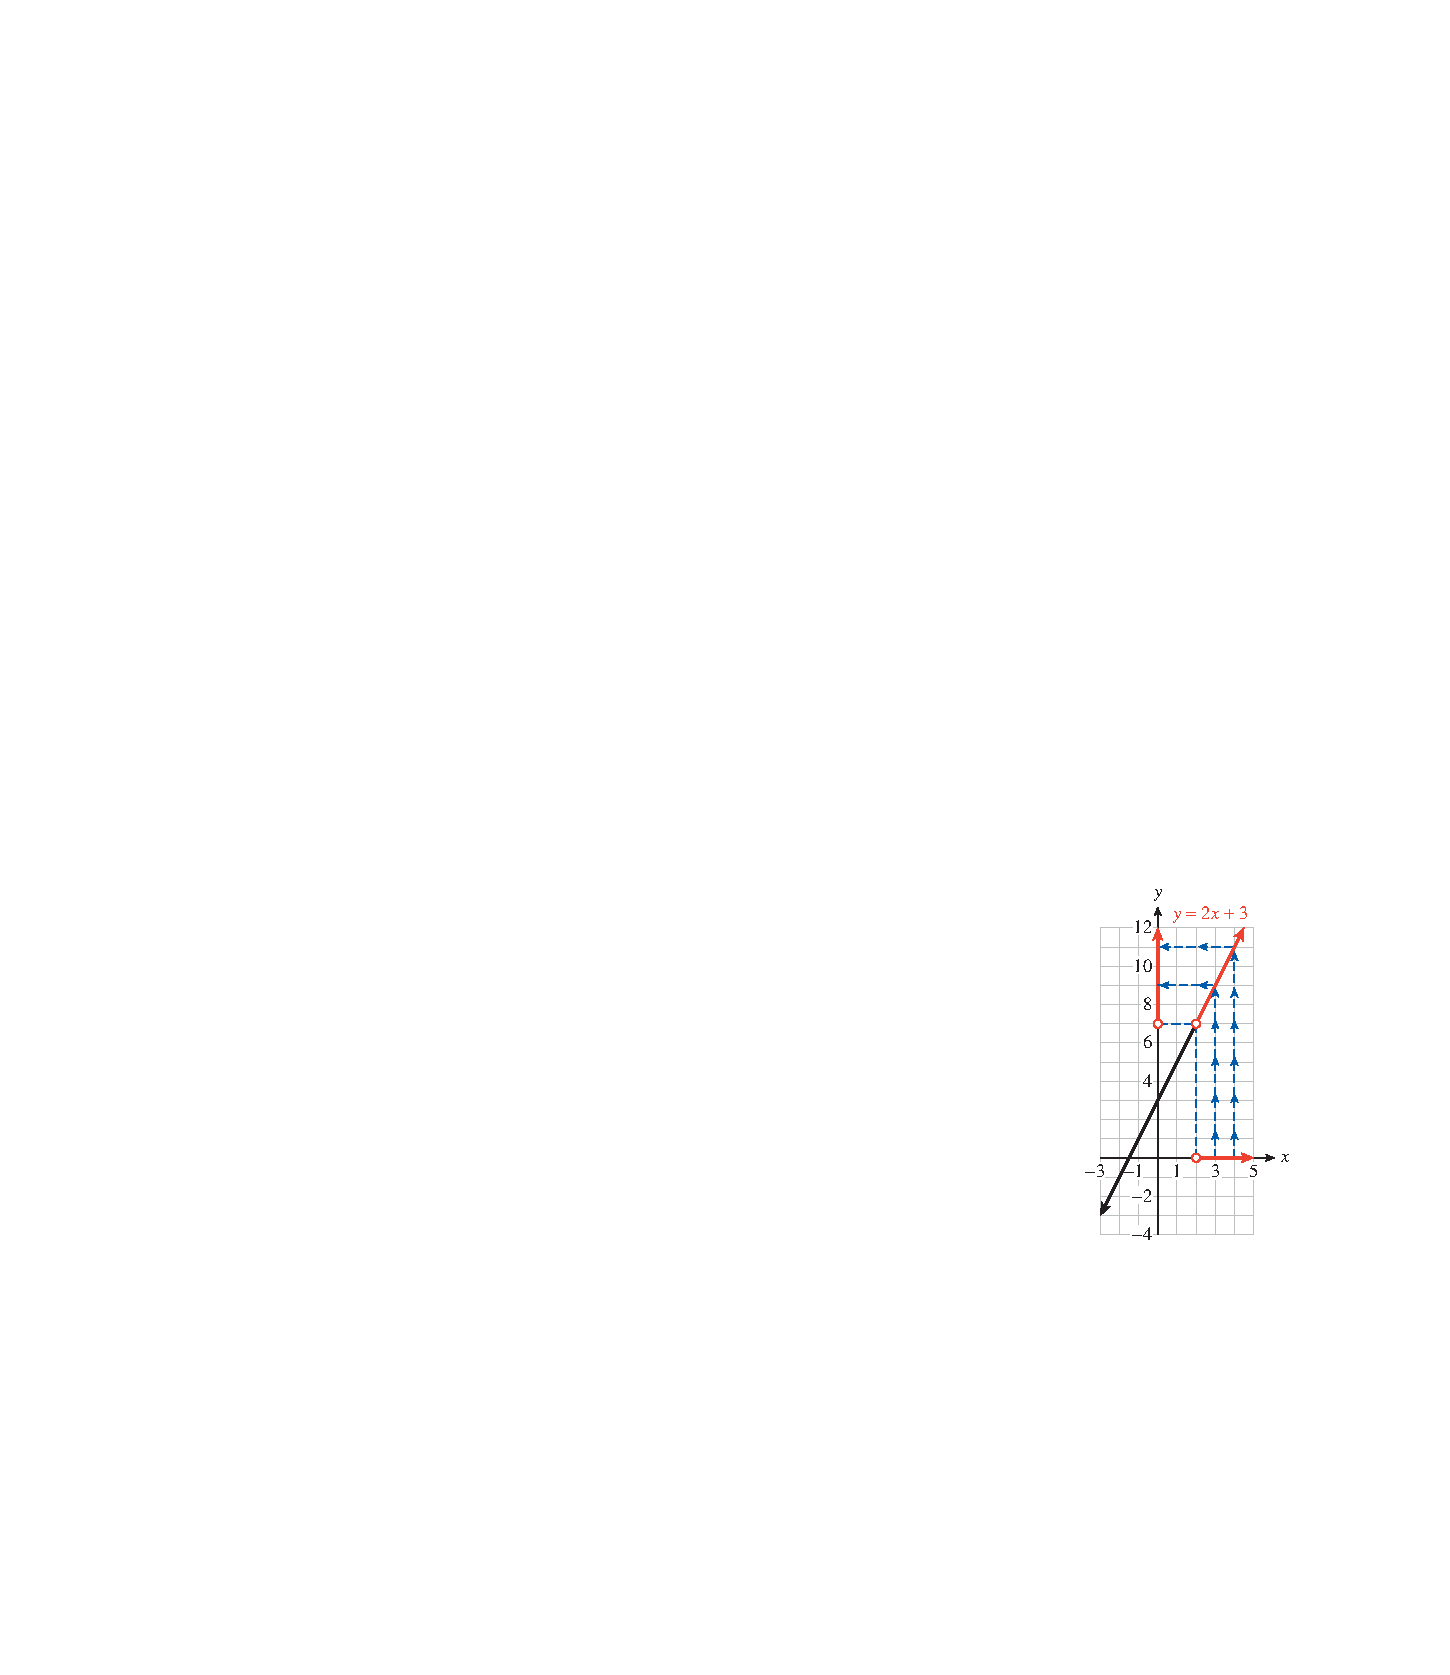
\includegraphics[width=\textwidth,]{images/fig-graph-to-solve3.pdf}}% end body 
{\captionof{figure}{\label{fig-graph-to-solve3}}
}% caption 
\popValignCaptionBottom
\end{figure}
\begin{example}[]\label{example-graph-to-solve2}
Use the graph of \(y = 285 − 15x\) to solve the inequality \begin{equation*}285 − 15x \gt 150\end{equation*}%
\par\medskip\noindent%
\textbf{Solution.}\quad 
    We begin by locating the point \(P\) on the graph for which \(y = 150\) and \(x = 9\) (its \(x\)-coordinate). Now, because \(y = 285 − 15x\) for points on the graph, the inequality \(285 − 15x \gt 150\) is equivalent to \(y \gt 150\). So we are looking for points on the graph with \(y\)-coordinate greater than \(150\). These points are shown in \hyperref[fig-graph-to-solve-inequality]{Figure~\ref{fig-graph-to-solve-inequality}}. The \(x\)-coordinates of these points are the \(x\)-values that satisfy the inequality. From the graph, we see that the solutions are \(x \lt 9\).
\leavevmode%
\begin{figure}
\centering
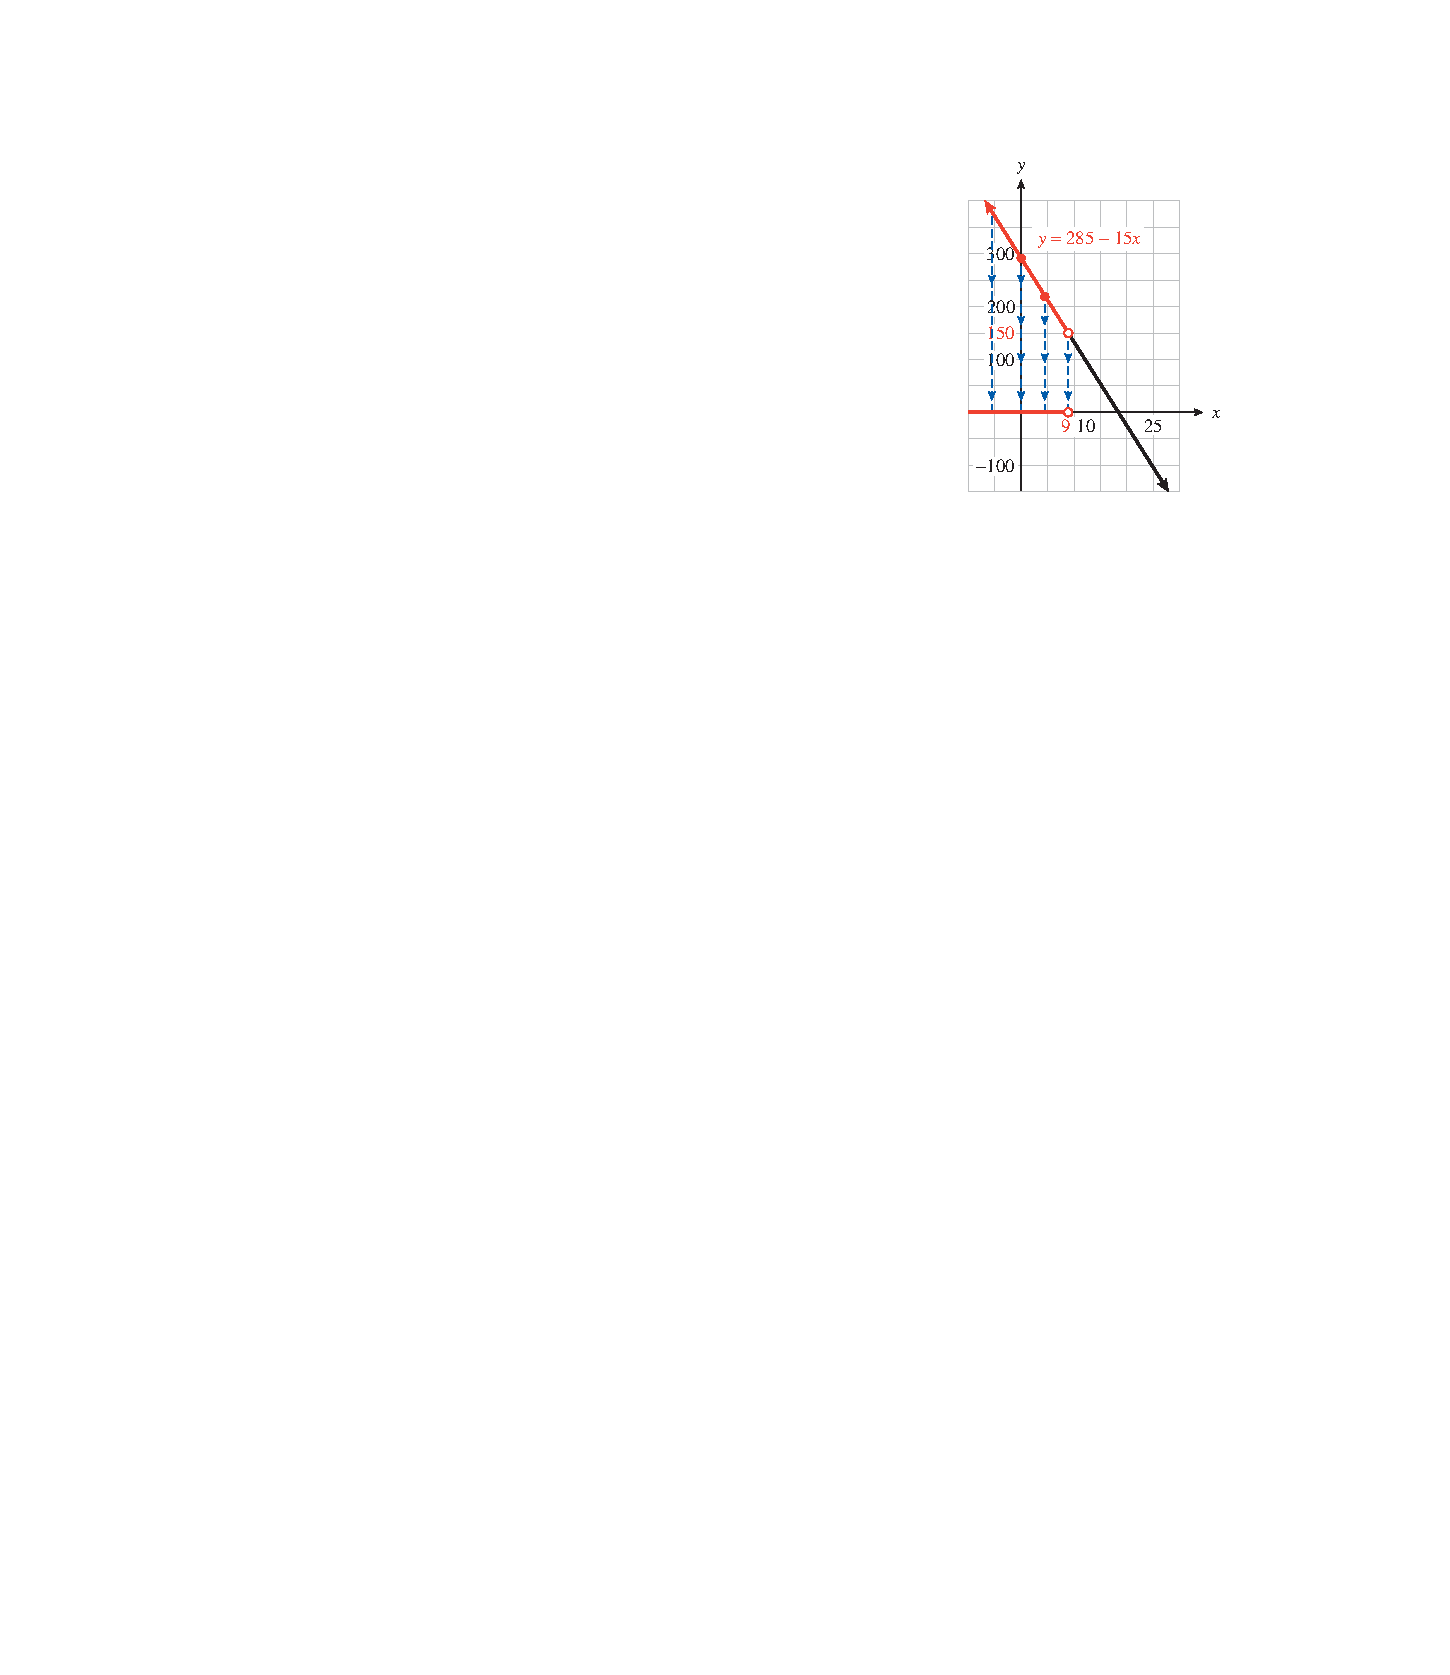
\includegraphics[width=0.60\textwidth,]{images/fig-graph-to-solve-inequality.pdf}\caption{\label{fig-graph-to-solve-inequality}}
\end{figure}
\end{example}
\begin{exercise}\label{exercise-graph-to-solve-inequality}
\leavevmode%
\begin{enumerate}[label=*\alph**]
\item\hypertarget{li-24}{}Use the graph of \(y = 30 − 8x\) in  \hyperref[fig-graph-to-solve2]{Figure~\ref{fig-graph-to-solve2}} to solve the inequality \begin{equation*}30 − 8x \le 50\end{equation*}\item\hypertarget{li-25}{}Solve the inequality algebraically.\end{enumerate}
\end{exercise}
\par
We can also use this graphical technique to solve nonlinear equations and inequalities.%
\begin{example}[]\label{example-graph-to-solve-cubic}
Use a graph of \(f(x) = −2x^3 + x^2 + 16x\) to solve the equation 
    \begin{equation*}−2x^3 + x^2 + 16x = 15\end{equation*}%
\par\medskip\noindent%
\textbf{Solution.}\quad If we sketch in the horizontal line \(y = 15\), we can see that there are three points on the graph of \(f\) that have \(y\)-coordinate \(15\), as shown in \hyperref[fig-graph-to-solve-cubic]{Figure~\ref{fig-graph-to-solve-cubic}}. The \(x\)-coordinates of these points are the solutions of the equation %
\leavevmode%
\begin{figure}
\centering
\pushValignCaptionBottom[b]{minipage}{.50\textwidth}{%
\parbox{\textwidth}{%
% horizontal alignment 
\begin{equation*}−2x^3 + x^2 + 16x = 15\end{equation*}
    From the graph, we see that the solutions are \(x = −3\), \(x = 1\), and approximately \(x = 2.5\). We can verify the solutions algebraically. For example, if \(x = \alert{−3}\), we have 
    \begin{align*}
        f(\alert{−3})\&−2(\alert{−3})3 + (\alert{−3})^2 + 16(\alert{−3})\textbackslash{}\textbackslash{}
        \&= −2(−27) + 9 − 48\textbackslash{}\textbackslash{}
        \&=54 + 9 − 48 = 15  
    \end{align*}
    so \(−3\) is a solution.}%
}% end body 
{}% caption 
\pushValignCaptionBottom[b]{minipage}{.50\textwidth}{%
\centering% horizontal alignment 
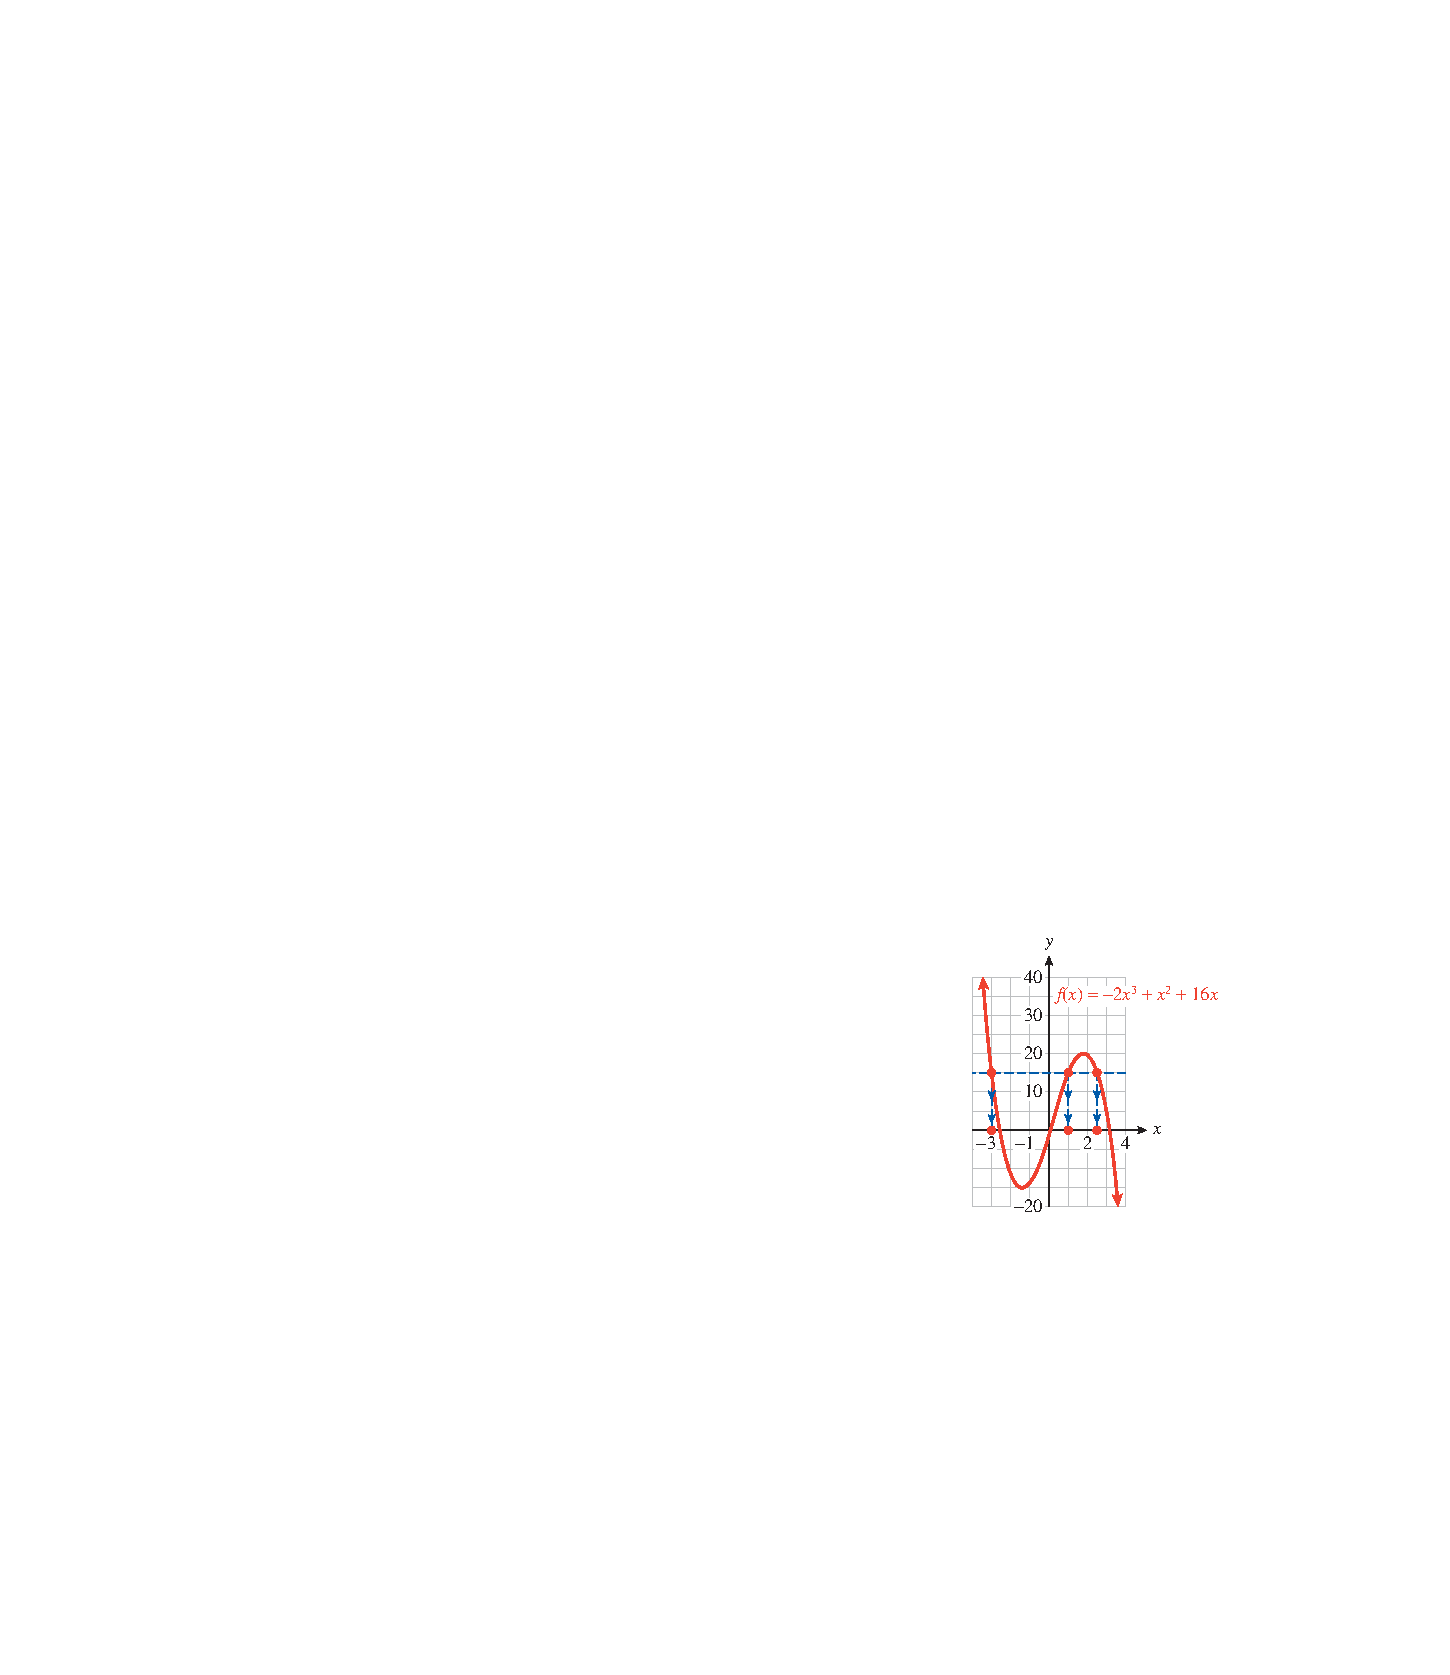
\includegraphics[width=\textwidth,]{images/fig-graph-to-solve-cubic.pdf}}% end body 
{\captionof{figure}{\label{fig-graph-to-solve-cubic}}
}% caption 
\popValignCaptionBottom
\end{figure}
\end{example}
\begin{exercise}\label{exercise-graph-to-solve-quadratic}

    Use the graph of \(y = \frac{1}{2}n^2 + 2n − 10\) shown in \hyperref[fig-graph-to-solve-quadratic]{Figure~\ref{fig-graph-to-solve-quadratic}} to solve
    \begin{equation*}\frac{1}{2}n^2 + 2n − 10 = 6\end{equation*}
    and verify your solutions algebraically.
\leavevmode%
\begin{figure}
\centering
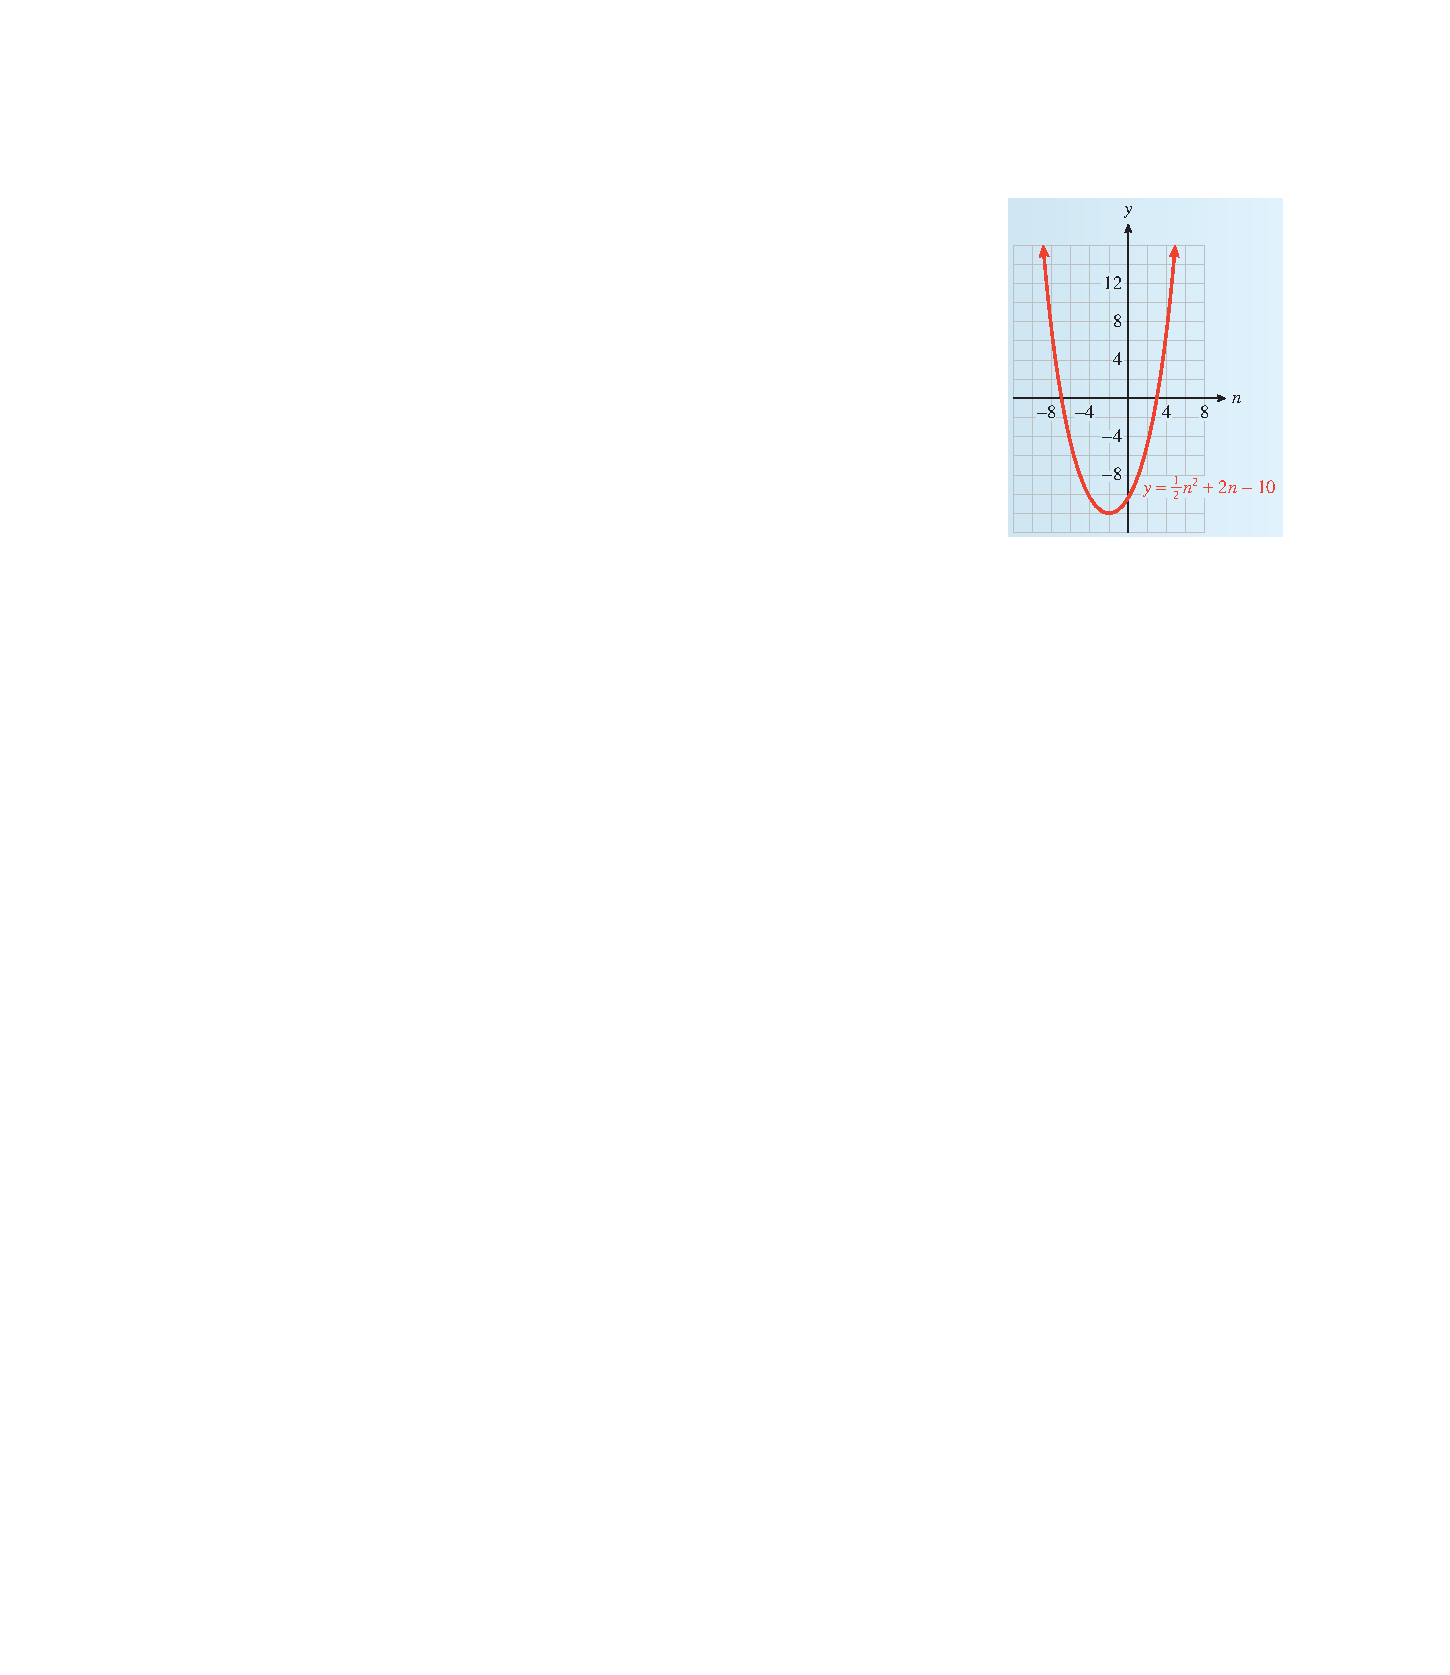
\includegraphics[width=0.60\textwidth,]{images/fig-graph-to-solve-quadratic.pdf}\caption{\label{fig-graph-to-solve-quadratic}}
\end{figure}
\end{exercise}
\begin{remark}[
\includegraphics[width=0.8\textwidth,]{images/icon-GC.pdf}Using the Trace Feature]\label{remark-3}
You can use the Trace feature on a graphing calculator to approximate solutions to equations. Graph the function \(f(x)\) in \hyperref[example-graph-to-solve-cubic]{Example~\ref{example-graph-to-solve-cubic}}  in the window
    \leavevmode%
\begin{table}
\centering
\begin{tabular}{lll}
Xmin\(=-4\)&&Xmax\(=4\)\tabularnewline[0pt]
Ymin\(=-20\)&&Ymax\(=40\)
\end{tabular}
\end{table}

    and trace along the curve to the point \((2.4680851, 15.512401)\). We are close to a solution, because the \(y\)-value is close to \(15\). Try entering \(x\)-values close to \(2.4680851\), for instance, \(x = 2.4\) and \(x = 2.5\), to find a better approximation for the solution.
%
\par

    We can use the intersect feature on a graphing calculator to obtain more accurate estimates for the solutions of equations. See {$\langle\langle$appendix-b$\rangle\rangle$} for details.
%
\end{remark}
\begin{example}[]\label{example-graph-to-solve-cubic2}
Use the graph in \hyperref[example-graph-to-solve-cubic]{Example~\ref{example-graph-to-solve-cubic}}  to solve the inequality
    \begin{equation*}−2x^3 + x^2 + 16x \ge 15\end{equation*}%
\par\medskip\noindent%
\textbf{Solution.}\quad 
        We first locate all points on the graph that have \(y\)-coordinates greater than or equal to \(15\). The \(x\)-coordinates of these points are the solutions of the inequality. \hyperref[fig-graph-to-solve-cubic2]{Figure~\ref{fig-graph-to-solve-cubic2}} shows the points, and their \(x\)-coordinates as intervals on the \(x\)-axis. The solutions are \(x \le −3\) and \(1\le x \le 2.5\), or in interval notation, \((-∞, −3] ∪ [1, 2.5]\).
        \leavevmode%
\begin{figure}
\centering
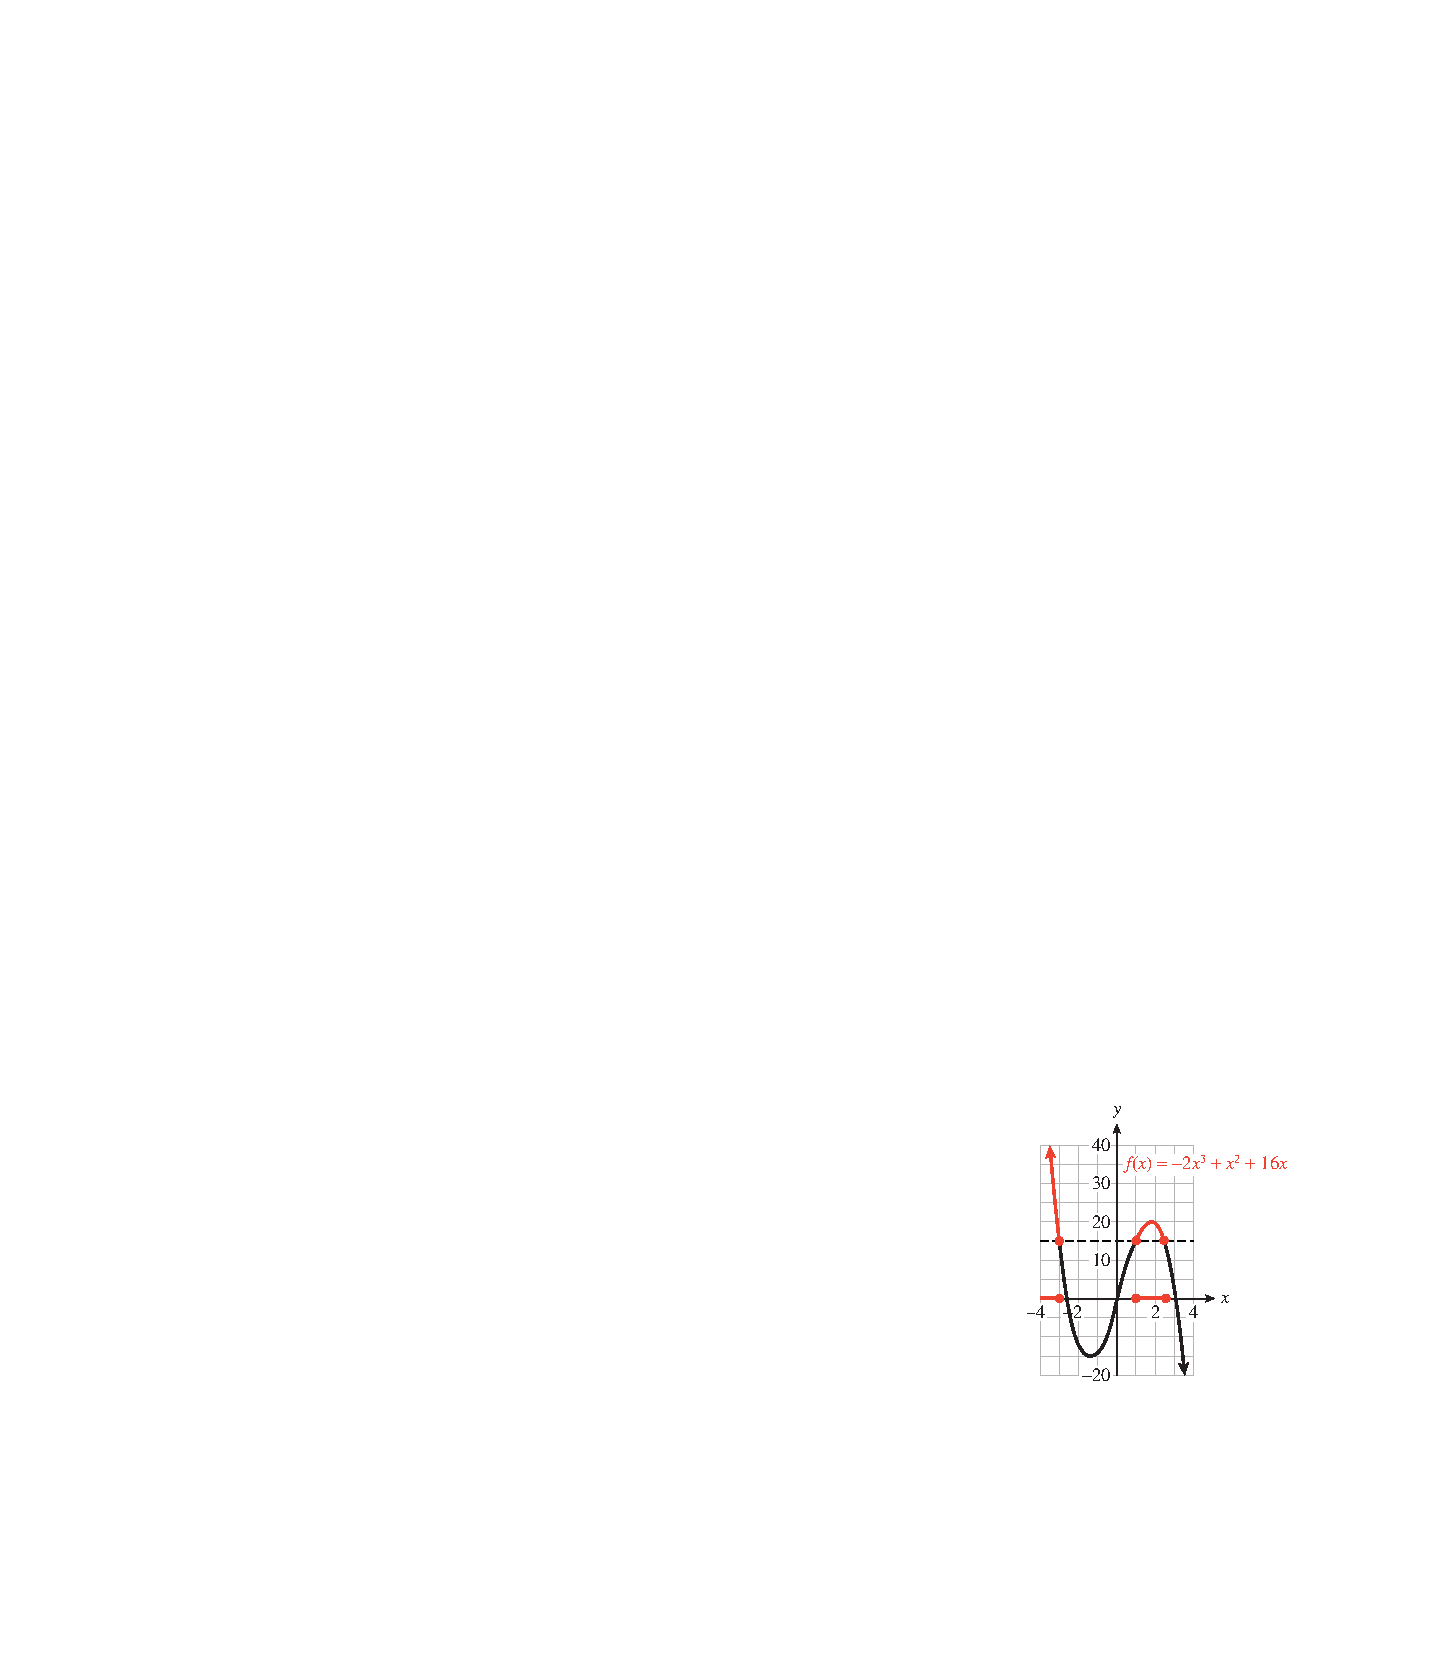
\includegraphics[width=0.60\textwidth,]{images/fig-graph-to-solve-cubic2.pdf}\caption{\label{fig-graph-to-solve-cubic2}}
\end{figure}
\end{example}
\begin{exercise}\label{exercise-graph-to-solve-quadratic2}
Use \hyperref[fig-graph-to-solve-quadratic]{Figure~\ref{fig-graph-to-solve-quadratic}} in \hyperref[exercise-graph-to-solve-quadratic]{Exercise~\ref{exercise-graph-to-solve-quadratic}} to solve the inequality
    \begin{equation*}\frac{1}{2}n^2 + 2n − 10 \lt 6\end{equation*}\end{exercise}
\typeout{************************************************}
\typeout{Section 1.2 Domain and Range}
\typeout{************************************************}
\section[Domain and Range]{Domain and Range}\label{Domain-Range}
\typeout{************************************************}
\typeout{Subsection 1.2.1 Definitions of Domain and Range}
\typeout{************************************************}
\subsection[Definitions of Domain and Range]{Definitions of Domain and Range}\label{subsection-5}

    In \hyperref[example-graph-square-root]{Example~\ref{example-graph-square-root}} of \hyperref[graphs-of-functions]{Section~\ref{graphs-of-functions}}, we graphed the function \(f (x) =\sqrt{x + 4}\) and observed that \(f (x)\) is undefined for \(x\)-values less than \(−4\). For this function, we must choose \(x\)-values in the interval \([−4, \infty)\). 
%
\leavevmode%
\begin{figure}
\centering
\pushValignCaptionBottom[b]{minipage}{.50\textwidth}{%
\centering% horizontal alignment 
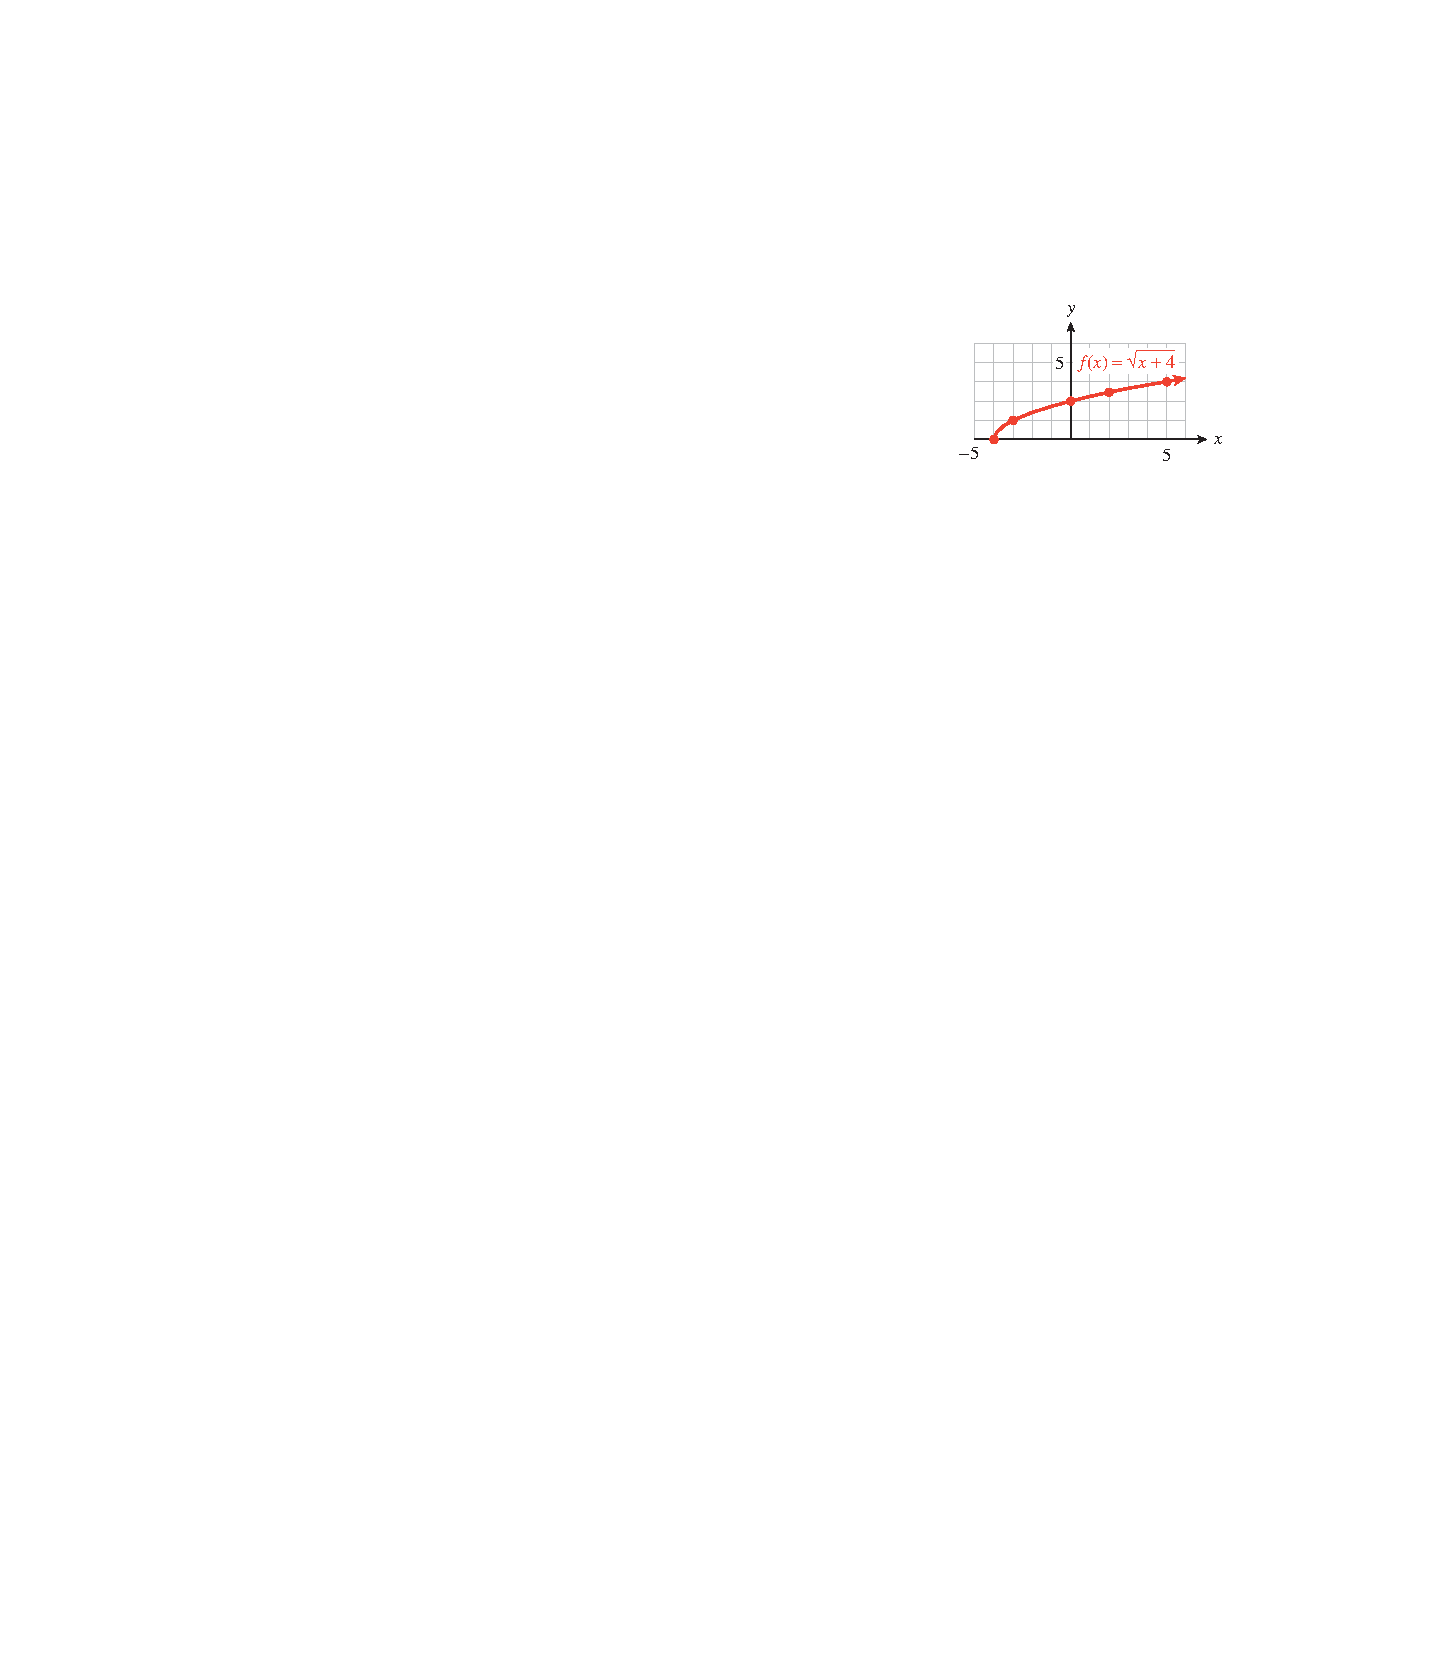
\includegraphics[width=\textwidth,]{images/fig-sq-root.pdf}}% end body 
{\captionof{figure}{\label{fig-sq-root-again}}
}% caption 
\pushValignCaptionBottom[b]{minipage}{.50\textwidth}{%
\parbox{\textwidth}{%
% horizontal alignment 

    All the points on the graph have \(x\)-coordinates greater than or equal to \(−4\), as shown in \hyperref[fig-sq-root-again]{Figure~\ref{fig-sq-root-again}}. The set of all permissible values of the input variable is called the \terminology{domain} of the function \(f\).
}%
}% end body 
{}% caption 
\popValignCaptionBottom
\end{figure}
\par

    We also see that there are no points with negative \(f (x)\)-values on the graph of \(f\): All the points have \(f (x)\)-values greater than or equal to zero. The set of all outputs or function values corresponding to the domain is called the \terminology{range} of the function. Thus, the domain of the function \(f (x) =\sqrt{x + 4}\) is the interval \([−4, \infty)\), and its range is the interval \([0, \infty)\). In general, we make the following definitions.
%
\typeout{************************************************}
\typeout{Paragraphs  Domain and Range}
\typeout{************************************************}
\paragraph[Domain and Range]{Domain and Range}\label{paragraphs-3}
%
\par

    The \terminology{domain} of a function is the set of permissible values for the input variable. The \terminology{range} is the set of function values (that is, values of the output variable) that correspond to the domain values.
%
\par

    Using the notions of domain and range, we restate the definition of a function as follows.
%
\typeout{************************************************}
\typeout{Paragraphs  Definition of Function}
\typeout{************************************************}
\paragraph[Definition of Function]{Definition of Function}\label{paragraphs-4}
%
\par

    A relationship between two variables is a \terminology{function} if each element of the domain is paired with exactly one element of the range.
%
\typeout{************************************************}
\typeout{Subsection 1.2.2 Finding Domain and Range from a Graph}
\typeout{************************************************}
\subsection[Finding Domain and Range from a Graph]{Finding Domain and Range from a Graph}\label{subsection-6}

    We can identify the domain and range of a function from its graph. The domain is the set of \(x\)-values of all points on the graph, and the range is the set of \(y\)-values.
%
\end{document}